% Notes and solutions


% -------------------------------------------------
% Package imports
% -------------------------------------------------
\documentclass[12pt, a4paper]{article}
\usepackage[utf8]{inputenc}% Input encoding
\usepackage[english]{babel}% Set language to english
\usepackage{graphicx}% For importing graphics
\usepackage{amsthm, amsfonts, amssymb, bm}% All the AMS packages
\usepackage{mathtools}% Fixes a few AMS bugs
\usepackage[expansion=false]{microtype}% Fixes to make typography better
\usepackage{hyperref}% For \href{URL}{text}
\usepackage{fancyhdr}% For fancy headers
\usepackage[sharp]{easylist}% Easy nested lists
\usepackage{parskip}% Web-like paragraphs
\usepackage{multicol}% For multiple columns
\usepackage{tikz-cd}% For diagrams
\usepackage{microtype}
\usepackage{listings}% To include source-code
\usepackage[margin = 2.5cm, includehead]{geometry}% May be used to set margins
\usepackage{nicefrac}% Enables \nicefrac{nom}{denom}
%\usepackage[sc]{mathpazo}% A nice font, alternative to CM
\usepackage{booktabs}

% -------------------------------------------------
% Package setup
% -------------------------------------------------

\newcommand{\Title}{Learning Machine Learning}
\newcommand{\Subtitle}{A summary of main ideas and concepts}
\newcommand{\Author}{tommyod}
\newcommand{\listSpace}{-0.5em}% Global list space

\title{\Title}
\author{\Author}

% Shortcuts for sets and other stuff in mathematics
\newcommand{\Q}{\mathbb{Q}}
\newcommand{\R}{\mathbb{R}}
\newcommand{\C}{\mathbb{C}}
\newcommand{\D}{\mathcal{D}}
\newcommand{\F}{\mathcal{F}}
\newcommand{\Y}{\mathcal{Y}}
\newcommand{\Reg}{\mathcal{R}}
\newcommand{\Class}{\mathcal{C}}
\newcommand{\Z}{\mathbb{Z}}
\renewcommand{\sf}[1]{\mathsf{#1}}
\newcommand{\vect}[1]{\bm{#1}}
\newcommand{\norm}[1]{\left\lVert#1\right\rVert}
\newcommand{\abs}[1]{\left\lvert#1\right\rvert}

% Shortcuts for probability distributions
\DeclareMathOperator{\N}{\mathcal{N}}
\DeclareMathOperator{\Bern}{\operatorname{Bern}}
\DeclareMathOperator{\Beta}{\operatorname{Beta}}
\DeclareMathOperator{\Bin}{\operatorname{Bin}}
\DeclareMathOperator{\St}{\operatorname{St}}
\DeclareMathOperator{\U}{\operatorname{U}}
\DeclareMathOperator{\KL}{\operatorname{KL}}

% Shortcuts for statistical operators
\DeclareMathOperator{\E}{\mathbb{E}}
\DeclareMathOperator{\var}{\operatorname{var}}
\DeclareMathOperator{\cov}{\operatorname{cov}}
\DeclareMathOperator{\SD}{\operatorname{SD}}
\renewcommand{\H}{\operatorname{H}}



% Change the section command to inluce lines, save space, etc.
%\usepackage{titlesec}
%\titlespacing\subsection{0pt}{6pt plus 4pt minus 2pt}{-0.8em plus 4pt minus 2pt}
%\titlespacing\paragraph{0pt}{6pt plus 4pt minus 2pt}{8pt plus 4pt minus 2pt}
%\titleformat{\section}
%{\normalfont\Large\bfseries}{\thesection}{0em}{$\vartriangleright$ }[{\titlerule[1.2pt]}]

% -------------------------------------------------
% Document start
% -------------------------------------------------
\begin{document}
	
\maketitle
\begin{abstract}
This document contains some notes and solutions to the book ``Pattern Classification'' by Duda et al.
\end{abstract}

\tableofcontents

\section{Notes from ``Pattern Recognition''}
\setcounter{subsection}{1}
\subsection{Bayesian Decision Theory}
\begin{easylist}[itemize]
\ListProperties(Space=\listSpace, Space*=\listSpace, Numbers1=l, FinalMark1={)})
# Bayes theorem is
\begin{equation*}
	P(\omega_j \mid \vect{x}) = \frac{p(\vect{x} \mid \omega_j) \times P(\omega_j)}{p(\vect{x})}
	= \frac{\text{likelihood} \times \text{prior}}{\text{evidence}}.
\end{equation*}
The Bayes decision rule is to choose $\omega_m$ such that
\begin{equation*}
	\omega_m = \arg \max_j P(\omega_j \mid \vect{x}).
\end{equation*}

# Loss functions (or risk functions) with losses other than zero-one is possible.
 In general, we choose the action $\lambda$ to minimize the risk $R(\lambda \mid \vect{x})$.
 
# The normal density 
\begin{equation*}
	p(\vect{x} \mid \vect{\mu}, \vect{\Sigma}) = \frac{1}{(2 \pi)^{d/2} \abs{\vect{\Sigma}}^{1/2}} 
	\exp \left[ - \frac{1}{2} 
	\left( \vect{x} - \vect{\mu} \right)^T \vect{\Sigma}^{-1} 
	\left( \vect{x} - \vect{\mu} \right) \right]
\end{equation*}

is often analytically tractable, and closed form discriminant functions exist.

# If features $\vect{y}$ are missing, we integrate them out using the sum rule
\begin{equation*}
	p(\vect{x}) = \int p(\vect{x}, \vect{y}) \, d\vect{y} = \int p(\vect{x} \mid \vect{y}) p(\vect{y}) \, d\vect{y}.
\end{equation*}

# In Bayesian belief networks, influences are represented by means of a directed graph.
If $B$ is dependent on $A$, we add a directed edge $A \to B$ to the network.
\end{easylist}




\subsection{Maximum-likelihood and Bayesian parameter estimation}
\begin{easylist}[itemize]
\ListProperties(Space=\listSpace, Space*=\listSpace, Numbers1=l, FinalMark1={)})
# The maximum likelihood of a distribution $p(\vect{x} \mid \vect{\theta})$ is given by $\hat{\vect{\theta}} = \arg \max_{\vect{\theta}} p(\D \mid \vect{\theta})$,
assuming i.i.d. data points and maximizing the log-likelihood, we have
\begin{equation*}
	\hat{\vect{\theta}} = \arg \max \ln  p(\D \mid \vect{\theta}) = \ln  \prod_{i=1}^{n} p(\vect{x}_i \mid \vect{\theta})  .
\end{equation*}
Analytical solutions exist for the Gaussian, but in general maximum likelihood estimates may be biased in the sense that $\E_x[ \hat{\vect{\theta}} ] = \int \hat{\vect{\theta}} p(\vect{x}) \, d\vect{x} \neq \vect{\theta}$.

# In the Bayesian framework, the parameter $\vect{\theta}$ is expressed by a probability density function $p(\vect{\theta})$.
This is called the \emph{prior} distribution of $\vect{\theta}$, which is updated when new data is seen.
The result is the \emph{posterior} distribution
\begin{equation*}
	p(\vect{\theta} \mid \D)  
	= 
	\frac{p(\D \mid \vect{\theta}) p (\vect{\theta})}
	{p(\D)}
	= 
	\frac{p(\D \mid \vect{\theta}) p (\vect{\theta})}
	{\int p(\D \mid \vect{\theta}) p(\vect{\theta}) \, d \vect{\theta}}.
\end{equation*}
The estimate of $\vect{x}$ becomes
\begin{equation*}
	p(\vect{x} \mid \D) = \int p(\vect{x}, \vect{\theta} \mid \D) \, d\vect{\theta} =
	\int p(\vect{x} \mid \vect{\theta} , \D) p(\vect{\theta} \mid \D)  \, d\vect{\theta} =
	\int p(\vect{x} \mid \vect{\theta}) p(\vect{\theta} \mid \D)  \, d\vect{\theta},
\end{equation*}
which may be interpreted as a weighted average of models $p(\vect{x} \mid \vect{\theta})$, where $p(\vect{\theta} \mid \D)$ is the weight associated with the model.

# The Bayesian framework is analytically tractable when using Gaussians.
For instsance, we can compute $p(\vect{\mu} \mid \D)$ if we assume $p(\vect{\mu}) \sim \N(\vect{\mu}_0, \vect{\Sigma}_0)$.
The distribution $p(\vect{\mu})$ is called the \emph{conjugate prior} and $p(\vect{\mu} \mid \D)$ is a \emph{reproducing density}, since the normal prior transforms to a normal posterior (with different parameters) when new data is seen.

# In summary the Bayesian framework allows us to incorporate prior information, but the maximum-likelihood approach is simpler.
Maximum likelihood gives us $\hat{\vect{\theta}}$, but the Bayesian framework gives us $p(\vect{\theta} | \D)$---the full distribution.

# Principal Component Analysis (PCA) yields components useful for \emph{representation}.
The covariance matrix is diagonalized, and low-variance directions in the hyperellipsoid are eliminated.
The computation is performed using the SVD.

# Discriminant Analysis (DA) projects to a lower dimensional subspace with optimal \emph{discrimination} (and not representation).

# Expectation Maximization (EM) is an iterative algorithm for finding the maximum-likelihood when data is missing (or latent).

# A discrete, first order, hidden Markov model consists of a transition matrix $\vect{A}$ and an emission matrix $\vect{B}$.
The probability of transition from state $i$ to state $j$ is given by $a_{ij}$, and the probability that state $i$ emits signal $j$ is given by $b_{ij}$.
Three fundamental problems related to Markov models are:
## The evaluation problem - probability that $\vect{V}^T$ was emitted, given $\vect{A}$ and $\vect{B}$.
## The decoding problem - determine most likely sequence of hidden states $\vect{\omega}^T$, given emitted $\vect{V}^T$, $\vect{A}$ and $\vect{B}$.
## The learning problem -- determine $\vect{A}$ and $\vect{B}$ given training observations of $\vect{V}^T$ and a coarse model.

\end{easylist}




\subsection{Nonparametric techniques}
\begin{easylist}[itemize]
\ListProperties(Space=\listSpace, Space*=\listSpace, Numbers1=l, FinalMark1={)})
# Two conceptually different approaches are available for nonparametric pattern recognition: 
## Estimation of densities $p(\vect{x} \mid w_j)$, called the \emph{generative} approach.
## Estimation of $P(w_j \mid \vect{x})$, called the \emph{discriminative} approach.

# Parzen-windows (kernel density estimation) is a generative method. 
It places a \emph{kernel function} $\phi: \R \to \R_+$ on every data point $\vect{x}_i$ to create a density estimate
\begin{equation*}
	p_n(\vect{x}) = \frac{1}{n} \sum_{i=1}^{n} \frac{1}{V_n} 
	\phi \left( \frac{\norm{\vect{x} - \vect{x}_i}_p}{h_n}  \right),
\end{equation*}
where $\norm{\cdot}: \R \times \R \to \R_+$ is metric defined by the $p$-norm (called the \emph{Minkowski metric}) and $h_n$ is the bandwidth.

# $k$-nearest neighbors is a discriminative method.
It uses information about the $k$ nearest neighbors to compute $P(w_j \mid \vect{x})$.
This automatically uses more of the surrounding space when data is sparse, and less of the surrounding space when data is dense.
The estimate $k$-nearest neighbor estimate is given by
\begin{equation*}
	P(w_j \mid \vect{x}) = \frac{\text{\# samples labeled } w_j}{k}.
\end{equation*}

# The \emph{nearest neighbor method} uses $k= 1$.
It can be shown that the error rate $P$ of the nearest neighbor method is never more than twice the Bayes error rate $P^*$ in the limit of infinite data.
More precisely, we have $P^* \leq P \leq P^* (2 - \frac{c}{c-1} P^*)$.

# In some applications, careful thought must be put into metrics.
Examples include periodic data on $\R / \Z$, and image data which where the metric should be invariant to shifts and small rotations.
One method to alleviate the problems of using the $L_2$ metric on images is to introduce the \emph{tangent distance}.
For an image $\vect{x}'$, the tangent vector of a transformation $\F$ (such as rotation by an angle $\alpha_i$) is
\begin{equation*}
	\vect{TV}_i = \F\left(\vect{x}'; \alpha_i \right) - \vect{x}'.
\end{equation*}
If several transformations are available, their linear combination may be computed.
For each test point $\vect{x}$, we search the tangent space the linear  combination minimizing the metric.
This gives information about $D(\vect{x}, \vect{x}')$ which is more invariant to transformations such as rotation and translation.

# Reduced Coloumb energy networks use ideas from both Parzen windows and $k$-nearest neighbors.
It adjusts the size of the window so that it is less than some maximal radius, while not touching any observation of a different class.
This creates ``basins of attraction'' for classification.
\end{easylist}


\subsection{Linear discriminant functions}
\begin{easylist}[itemize]
\ListProperties(Space=\listSpace, Space*=\listSpace, Numbers1=l, FinalMark1={)})
# Linear discriminant functions split the feature space in two with a hyperplance, which is defined as
\begin{equation*}
	g(x) = \omega^T x + \omega_0 = a^T y =
	\begin{pmatrix}
	\omega_0 & \omega
	\end{pmatrix}
	\begin{pmatrix}
	1 \\
	x
	\end{pmatrix},
\end{equation*}
where in the first form $\omega_0$ is the bias. The second form is the \emph{augmented} form.

# A linear machine assigns a point $x$ to $\omega_i$ if
\begin{equation*}
	g_i( x ) \geq g_j( x )
\end{equation*}
for every other class $j$.
This leaves no ambiguous regions in the feature space.

# Introducing mappings $y = h(x)$ to higher dimensional spaces, non-linearities in $x$-space may be captured by linear classifiers working in $y$ space. An example is $h(x) = \exp(-x^T x)$ if data from one class i centered around the origin.

# Several algorithms may be used to decrease an error function.
Two choices are gradient descent and Newton descent.
## Gradient descent moves in the direction of the negative gradient.
It is often controlled by a step length parameter $\eta(k)$, which may decrease as the iterations $k$ increase.
\begin{equation*}
	\vect{a} \leftarrow \vect{a} - \eta(k) \nabla J(\vect{a})
\end{equation*}
## Newton descent also moves in the direction of the negative gradient, but the optimal step length is computed by linearizing the function $\nabla J(\vect{a})$ (or, equivalently, a second order approximation of $\vect{a}$).
\begin{equation*}
\vect{a} \leftarrow \vect{a} - \vect{H}^{-1} \nabla J(\vect{a})
\end{equation*}

# Criterion functions for linearly separable data sets include:
## The Perceptron function $\sum_{y \in \Y} (-\vect{a}^T \vect{y})$, which is not smooth.
## The squared error with margin is $\sum_{y \in \Y} (\vect{a}^T \vect{y} - b)^2 / \norm{\vect{y}}^a$.

# MSE may be used, but does not in general yield a separating hyperplane---even if one exists.
## The MSE solutions is found analytically by the pseudoinverse $\vect{A}^\dagger = \left( \vect{A}^T \vect{A} \right)^{-1} \vect{A}^T$, which solves the least squares problem
\begin{equation*}
	\min_x \vect{e}^T\vect{e} = 
	\min_x \left(\vect{b} - \vect{A}\vect{x}\right)^T
	\left(\vect{b} - \vect{A}\vect{x}\right).
\end{equation*}
## Related to Fisher's linear discriminant for an appropriate choice of margin vector $\vect{b}$.
## LMS may be computed using matrix procedures (never use the pseudoinverse directly) or by the gradient descent algorithm.
## Ho-Kashyap procedures yield a separating hyperplane if one exists.

# \emph{Linear programming} (LP) may also be used to find a separating hyperplane. Several reductions are possible by introduction of \emph{artificial variables}.
## Minimizing the Perceptron criterion function may be formulated as LP, and the result is decent even if a separating hyperplane does not exist.

# \emph{Support Vector Machines} (SVM) find the minimum margin hyperplane.
This is a quadratic programming (QP) problem, and the dual problem is easier to solve than the primal problem.
\end{easylist}


\subsection{Multilayer Neural Networks}
\begin{easylist}[itemize]
\ListProperties(Space=\listSpace, Space*=\listSpace, Numbers1=l, FinalMark1={)})
# TODO
\end{easylist}




\clearpage
\section{Solutions to ``Pattern Recognition''}

\setcounter{subsection}{1}
\subsection{Bayesian Decision Theory}

\subsubsection*{Problem 2.6}
\begin{easylist}[enumerate]
\ListProperties(Space=\listSpace, Space*=\listSpace, Numbers1=l, FinalMark1={)})
# We want the probability of choosing action $\alpha_2$ to be smaller than, or equal to, $E_1$, given that the true state of nature is $\omega_1$.
Let's assume that $\mu_1 < \mu_2$ and that the decision threshold is $x^*$, so we decide $\alpha_2$ if $x > x^*$.
We then have
\begin{align*}
	P(\alpha_2 | \omega_1) &\leq E_1 \\
	p(x > x^* | \omega_1) &\leq E_1 \\
	\left[1 - \int_{0}^{x^*} p(x | \omega_1)  \, dx \right] &\leq E_1
\end{align*}
We let $\Phi: \R \to \left[0, 1\right]$ denote the cumulative Gaussian distribution, and $\Phi^{-1}: \left[0, 1\right] \to \R$ it's inverse function.
Making use of $\Phi$ we write
\begin{align*}
1 - \Phi \left( \frac{x^* - \mu_1}{\sigma_1} \right) &\leq E_1 \\
x^* \geq \mu_1 + \sigma_1 \Phi^{-1} \left(1 - E_1 \right).
\end{align*}
If the desired error is close to zero, then $x^*$ goes to positive infinity.
If the desired error is close to one, then $x^*$ goes to negative infinity.

# The error rate for classifying $\omega_2$ as $\omega_1$ is
\begin{equation*}
	P(\alpha_1 | \omega_2) = 	p(x \leq x^* | \omega_2) = \int_{0}^{x^*} p(x| \omega_2) \, dx 
	= 
	\Phi \left(  \frac{x^* - \mu_2}{\sigma_2}  \right).
\end{equation*}
Making use of $x^*$ from the previous problem, we obtain
\begin{equation*}
 \Phi \left(  \frac{ \mu_1 + \sigma_1 \Phi^{-1} \left(1 - E_1 \right) - \mu_2}{\sigma_2}  \right) 
 =
\Phi \left(  \frac{\mu_1 - \mu_2}{\sigma_2} + \frac{\sigma_1}{\sigma_2}  \Phi^{-1} \left(1 - E_1 \right) \right).
\end{equation*}
# The overall error rate becomes
\begin{align*}
	P(\text{error}) &= P(\alpha_1, \omega_2) + P(\alpha_2, \omega_1) \\
	&= P(\alpha_1 | \omega_2) P(\omega_2) + P(\alpha_2| \omega_1) P(\omega_1) \\
	&= \frac{1}{2} \left[  P(\alpha_1 | \omega_2) +  P(\alpha_2| \omega_1) \right] \\
	&= \frac{1}{2} \left[ E_1 +  \Phi \left(  \frac{\mu_1 - \mu_2}{\sigma_2} + \frac{\sigma_1}{\sigma_2}  \Phi^{-1} \left(1 - E_1 \right) \right) \right].
\end{align*}
In the last equality we used the results from the previous problems.

# We substitute the given values into the equations, and obtain $x^* \approx 0.6449$. The total error rate is $P(\text{error}) \approx 0.2056$.
# The Bayes error rate, as a function of $x^*$, is given by
\begin{align*}
	P(\text{error}) = P(\alpha_2 | \omega_1) P(\omega_1) + P(\alpha_1| \omega_2) P(\omega_2) \\
	= \frac{1}{2} \left[ p( x > x^*| \omega_1)  + p( x < x^* | \omega_2) \right]   \\
	= \frac{1}{2} \left[ \left( 1 - \Phi \left( \frac{x^* - \mu_1}{\sigma_1}\right)\right) +  \Phi \left( \frac{x^* - \mu_2}{\sigma_2}\right)  \right]
\end{align*}
The Bayes error rate is depicted in Figure \ref{fig:duda_ch2_prob6}.

\begin{figure}[ht!]
\centering
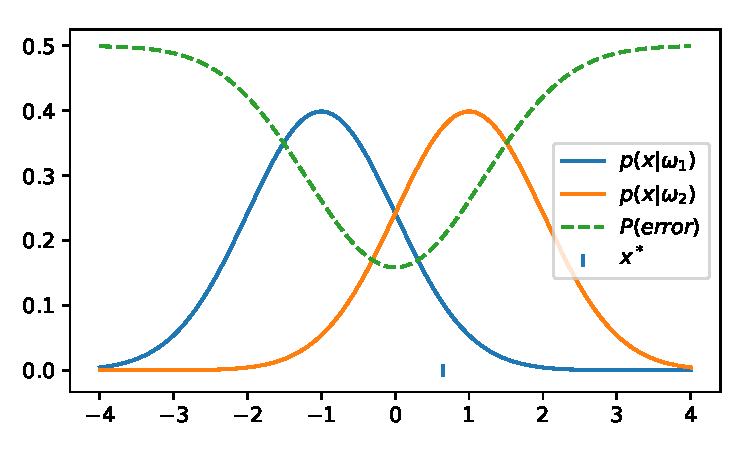
\includegraphics[width=0.5\linewidth]{figs/duda_ch2_prob6}
\caption{Graf accompanying problem 2.6.}
\label{fig:duda_ch2_prob6}
\end{figure}


\end{easylist}

\subsubsection*{Problem 2.12}
\begin{easylist}[enumerate]
\ListProperties(Space=\listSpace, Space*=\listSpace, Numbers1=l, FinalMark1={)})
# The key observation is that the maximal value $P(\omega_{\text{max}} | \vect{x} )$ is greater than, or equal to, the average. Therefore we obtain
\begin{equation*}
	P(\omega_{\text{max}} | \vect{x} ) \geq \frac{1}{c} \sum_{i=1}^{c} P(\omega_i | \vect{x}) = \frac{1}{c},
\end{equation*}
where the last equality is due to probabilities summing to unity.
# The minimum error rate is achieved by choosing $\omega_{\text{max}}$, the most likely state of nature. 
The average probability of error over the data space is therefore the probability that $\omega_{\text{max}}$ is \emph{not} the true state of nature for a given $\vect{x}$, that is:
\begin{equation*}
	P(\text{error}) = \E_x \left[ 1 - P(\omega_{\text{max}} | \vect{x} ) \right] = 1 - \int P(\omega_{\text{max}} | \vect{x} ) p(\vect{x}) \, d \vect{x}.
\end{equation*}

# We see that
\begin{equation*}
	P(\text{error}) = 1 - \int P(\omega_{\text{max}} | \vect{x} ) p(\vect{x}) \, d \vect{x} \leq 1 - \int \frac{1}{c} p(\vect{x}) \, d \vect{x} = 1 - \frac{1}{c} = \frac{c-1}{c},
\end{equation*}
where we used $\int p(\vect{x}) \, d \vect{x} = 1$.


# A situation where $P(\text{error}) = (c-1)/c$ arises when $P(\omega_i) = 1/c$ for every $i$. Then the maximum value is equal to the average value, and the inequality in problem a) becomes an equality.
\end{easylist}


\subsubsection*{Problem 2.19}
\begin{easylist}[enumerate]
\ListProperties(Space=\listSpace, Space*=\listSpace, Numbers1=l, FinalMark1={)})
# The entropy is given by $\H\left[p(x)\right] = - \int p(x) \ln p(x) \, dx$.
The optimization problem gives the synthetic function
\begin{align*}
	H_s = - \int p(x) \ln p(x) \, dx + \sum_{k=1} ^{q} \lambda_k \left( \int b_k(x) p(x) \, dx - a_k \right),
\end{align*}
and since a probability density function has $\int p(x) \, dx = 1$ we add an additional constraint for $k=0$ with $b_0(x) = 1$ and $a_k = 1$.
Collecting terms we obtain
\begin{align*}
H_s &= - \int p(x) \ln p(x) \, dx + \sum_{k=0} ^{q} \lambda_k  \int b_k(x) p(x) \, dx - \sum_{k=0} ^{q} \lambda_k a_k  \\
&= - \int p(x) 
\left[ \ln p(x) - \sum_{k=0} ^{q} \lambda_k b_k(x) \right] \, dx - \sum_{k=0} ^{q} \lambda_k a_k ,
\end{align*}
which is what we were asked to show.
# Differentiating the equation above with respect to $p(x)$ and equating it to zero we obtain
\begin{equation*}
	- \int \left(  1 \left[ \ln p(x) - \sum_{k=0} ^{q} \lambda_k b_k(x) \right] + p(x) \left[ \frac{1}{p(x)} \right] \right) \, dx = 0.
\end{equation*}
This integral is zero if the integrand is zero for every $x$, so we require that
\begin{equation*}
	 \ln p(x) - \sum_{k=0} ^{q} \lambda_k b_k(x) + 1 = 0,
\end{equation*}
and solving this equation for $p(x)$ gives the desired answer.
\end{easylist}

\subsubsection*{Problem 2.21}
We are asked to compute the entropy of the (1) Gaussian distribution, (2) triangle distribution and (3) uniform distribution. 
Every p.d.f has $\mu = 0$ and standard deviation $\sigma$, and we must write every p.d.f parameterized using $\sigma$.
\paragraph{Gaussian} We use the definition $\H\left[p(x)\right] = - \int p(x) \ln p(x) \, dx$ to compute  
\begin{equation*}
	\H\left[p(x)\right] = 
	- \int \frac{1}{\sqrt{2 \pi} \sigma} 
	\exp \left( - \frac{1}{2} \frac{x^2}{\sigma^2} \right) 
	\left[ \ln \left( \frac{1}{\sqrt{2 \pi} \sigma } \right) - \frac{1}{2} \frac{x^2}{\sigma^2} \right] \, dx.
\end{equation*}
Let us denote $K = \frac{1}{\sqrt{2 \pi} \sigma} $ to simplify notation. We obtain
\begin{align*}
	- \int & K
	\exp \left( - \frac{1}{2} \frac{x^2}{\sigma^2} \right) 
	\left[ \ln K - \frac{1}{2} \frac{x^2}{\sigma^2} \right] \, dx = \\
	- K \ln K \int & 
	\exp \left( - \frac{1}{2} \frac{x^2}{\sigma^2} \right) \, dx + K \int  \frac{1}{2} \frac{x^2}{\sigma^2} \exp \left( - \frac{1}{2} \frac{x^2}{\sigma^2} \right)  \, dx
\end{align*}
The first term is simply negative $\ln K$, since it's the normal distribution with an additional factor $-\ln K$.
The second term is not as straightforward.
We change variables to $y = x / \left( \sqrt{2} \sigma \right)$, and write it as
\begin{equation*}
	K \int  y^2 \exp \left( - y^2 \right) \sqrt{2} \sigma \, dy,
\end{equation*}
which can be solved by using the following observation (from integration by parts)
\begin{equation*}
	\int 1 e^{-x^2} \, dx = \underbrace{\left. x e^{-x^2} \right|}_{0\text{ at } \pm \infty} - \int x (-2x) e^{-x^2} \, dx.
\end{equation*}
Using the above equation in reverse, we integrate as follows:
\begin{equation*}
	K \sqrt{2} \sigma \int  y^2 \exp \left( - y^2 \right)  \, dy = 	K \sqrt{2} \sigma \frac{1}{2}\int  \exp \left( - y^2 \right)  \, dy = K \sqrt{2} \sigma \frac{1}{2} \sqrt{\pi} = \frac{1}{2}
\end{equation*}
To recap, the first integral evaluated to $- \ln K$, and the second evaluated to $\frac{1}{2}$.
The entropy of the Gaussian is therefore $1/2 + \ln \sqrt{2 \pi } \sigma$.

\paragraph{Triangle}
The triangle distribution may be written in the form
\begin{equation*}
	f(x) = \begin{cases}
	h - \frac{hx}{b} &\quad \text{ if } \abs{x} < b\\
	0 &\quad \text{ if } \abs{x} \geq b,
	\end{cases}
\end{equation*}
where $h$ is the height and $b$ is the width to the left of, and to the right of, $x=0$.

Since the integral must evaluate to unity, we impose $hb = 1$ and obtain $f(x;b) = \frac{1}{b} \left( 1- \frac{x}{b}\right)$.
We wish to parameterize the triangle distribution using the standard deviation $\sigma$ instead of width $b$.
We can use $\var(X) = \E(X^2) - \E(X)^2$ to find the variance, since in this case $\E(X)^2 = \mu^2 = 0$ since the function is centered on $x=0$.
Computing $\E(X^2)$ yields $b^2 / 6$, so $b^2 = 6 \sigma^2$.
The revised triangle distribution then becomes
\begin{equation*}
f(x; \sigma) = \begin{cases}
\frac{1}{\sqrt{6} \sigma} \left(1 - \frac{x}{\sqrt{6} \sigma}\right) &\quad \text{ if } \abs{x} < \sqrt{6} \sigma \\
0 &\quad \text{ if } \abs{x} \geq \sqrt{6} \sigma .
\end{cases}
\end{equation*}
We set $k = \frac{1}{\sqrt{6} \sigma}$ to ease notation.
Due to symmetry, we compute the entropy as 
\begin{equation*}
	\H\left[f(x; \sigma)\right] = - 2 \int_{0}^{\sqrt{6} \sigma} k \left(1 - kx\right) \ln \left( k \left(1 - k x \right) \right) \, dx.
\end{equation*}
Changing variables to $y = 1 - kx$ we obtain
\begin{align*}
& - 2 \int_{x=0}^{x=\sqrt{6} \sigma} k y  \left( \ln k + \ln y \right) \, dx = - 2 \int_{y = 1}^{y = 0} k y  \left( \ln k + \ln y \right) \left(\frac{1}{-k}\right) \, dy \\
& - 2 \int_{0}^{1} y \left( \ln k + \ln y \right) dy = - 2 \int_{0}^{1} y \ln k \, dy - 2 \int_{0}^{1} y  \ln y \, dy = -2 \left( \ln k - \frac{1}{4}\right),
\end{align*}
where the last integral can be evaluated using integration by parts.
The entropy of the triangle distribution turns out to be $1/2 + \ln \sqrt{6} \sigma$.

\paragraph{Uniform}
Using the same logic as with the triangle distribution to normalize a uniform distribution, and then parameterizing by $\sigma$, we obtain
\begin{equation*}
u(x; \sigma) =
\left\{\!\begin{aligned}
\frac{1}{2b} &\quad \text{ if } \abs{x} < b \\
0 &\quad \text{ if } \abs{x} \geq b 
\end{aligned}\right\}
= 
\left\{\!\begin{aligned}
\frac{1}{2\sqrt{3}\sigma} &\quad \text{ if } \abs{x} <\sqrt{3}\sigma \\
0 &\quad \text{ if } \abs{x} \geq \sqrt{3}\sigma.
\end{aligned}\right.
\end{equation*}
Computing the entropy is easier than in the case of the Gaussian and the triangle distribution, we simply evaluate the integral as
\begin{equation*}
\H\left[p(x)\right] =2  \int_0^{\sqrt{3} \sigma} \frac{1}{2\sqrt{3}\sigma} \ln \frac{1}{2\sqrt{3}\sigma}  \, dx = \ln 2 \sqrt{3} \sigma.
\end{equation*}.

Let's briefly compare the results of our computations as follows:
\begin{align*}
	H_\text{Gaussian}(\sigma) &= 1/2 + \ln \sqrt{2 \pi } \sigma = \frac{1}{2} + \ln \sqrt{2\pi}  + \ln \sigma \approx 1.4189 + \ln \sigma \\
	H_\text{Triangle}(\sigma) &= 1/2 + \ln \sqrt{6} \sigma = \frac{1}{2} + \ln \sqrt{6} + \ln \sigma \approx 1.3959 + \ln \sigma \\
	H_\text{Uniform}(\sigma) &= \ln 2 \sqrt{3} \sigma = 0 + \ln 2 \sqrt{3} + \ln \sigma \approx 1.2425 + \ln \sigma
\end{align*}
This verifies that out of the three distributions, the Gaussian has the maximal entropy.
This was expected, since the Gaussian maximizes the entropy over \emph{any} continuous p.d.f. having a prescribed mean and variance.



\subsubsection*{Problem 2.23}
\begin{easylist}[enumerate]
\ListProperties(Space=\listSpace, Space*=\listSpace, Numbers1=l, FinalMark1={)})
# To solve this problem, we need to find the inverse matrix, the determinant, and $\vect{w} = \vect{x} - \vect{\mu}$.
\begin{equation*}
	\vect{\Sigma}^{-1} = \frac{1}{21}\begin{pmatrix}
	1 & 0 & 0 \\
	0 & 5 & -2 \\
	0 & -2 & 5 \\
	\end{pmatrix}
	\quad
	\det \vect{\Sigma} = 21
	\quad
	\vect{w} = \vect{x} - \vect{\mu} = 
	\begin{pmatrix}
	-0.5 \\
	-2 \\
	-1
	\end{pmatrix}
\end{equation*}
The number of dimension $d$ is 3.
The solution is
\begin{equation*}
	p(\vect{x}) = \frac{1}{\left(2 \pi \right)^\frac{3}{2} 21^{\frac{1}{2}}} \exp \left( -\frac{1}{2} \vect{w}^T \vect{\Sigma}^{-1} \vect{w}\right)
	= \frac{1}{\left(2 \pi \right)^\frac{3}{2} 21^{\frac{1}{2}}} \exp \left( -\frac{1}{2} \frac{1}{21} \frac{69}{4}\right).
\end{equation*}
# The eigenvalues of $\vect{\Sigma}$ are $\lambda_1 = 3$, $\lambda_1 = 7$ and $\lambda_1 = 21$.
The corresponding eigenvectors are
$\vect{v}_1 = (0, 1, -1)^T / \sqrt{2}$, 
$\vect{v}_2 = (0, 1, 1)^T / \sqrt{2}$ and 
$\vect{v}_3 = (1, 0, 0)^T$.
The whitening transformation is therefore given by
\begin{equation*}
	\vect{A}_w = \vect{\Phi} \vect{\Lambda}^{-1/2} = 
	\frac{1}{\sqrt{2}}
	\begin{pmatrix}
	0 & 0 & \sqrt{2} \\
	1 & 1 & 0 \\
	-1 & 1 & 0 \\
	\end{pmatrix}
	\begin{pmatrix}
	-\sqrt{3} & 0 & 0 \\
	0 & -\sqrt{7} & 0 \\
	0 & 0 & -\sqrt{21} 
	\end{pmatrix}.
\end{equation*}
The rest of the numerical computations are skipped.
# Skipped.
# Skipped.
# We are going to examine if the p.d.f is unchanged when vectors are transformed with $\vect{T}^T \vect{x}$ and matrices with $\vect{T}^T \vect{\Sigma} \vect{T}$.
Let's consider the term $\left(\vect{x} - \vect{\mu}\right)^T \vect{\Sigma}^{-1} \left(\vect{x} - \vect{\mu}\right)$ in the exponent first.
Substituting $\vect{x} \mapsto \vect{T}^T \vect{x}$,
$\vect{\mu} \mapsto \vect{T}^T \vect{\mu}$ and
$\vect{\Sigma} \mapsto \vect{T}^T \vect{\Sigma} \vect{T}$, we observe that
\begin{gather*}
	\left(\vect{T}^T\vect{x} - \vect{T}^T\vect{\mu}\right)^T
	 \left( \vect{\vect{T}^T\Sigma}\vect{T}  \right)^{-1}
	 \left(\vect{T}^T\vect{x} - \vect{T}^T\vect{\mu}\right) \\
	\left(\vect{T}^T\left(\vect{x} - \vect{\mu}\right)\right)^T
	 \left( \vect{\vect{T}^T\Sigma}\vect{T}  \right)^{-1}
	 \vect{T}^T\left(\vect{x} - \vect{\mu}\right) \\
	 \left(\vect{x} - \vect{\mu}\right)^T \vect{T}
	 \left( \vect{T}^T \vect{\Sigma}\vect{T}  \right)^{-1}
	 \vect{T}^T\left(\vect{x} - \vect{\mu}\right) \\
	 \left(\vect{x} - \vect{\mu}\right)^T \vect{T}
	 \vect{T}^{-1} \vect{\Sigma}^{-1}\vect{T}^{-T}
	 \vect{T}^T\left(\vect{x} - \vect{\mu}\right) \\
	 \left(\vect{x} - \vect{\mu}\right)^T 
	  \vect{\Sigma}^{-1}
	 \left(\vect{x} - \vect{\mu}\right),
\end{gather*}
where we have used $(\vect{A}\vect{B})^T = \vect{B}^T \vect{A}^T$ and $(\vect{A}\vect{B})^{-1} = \vect{B}^{-1} \vect{A}^{-1}$, which are basic facts from linear algebra.
The density remains proportional when applying a linear transformation, but not unscaled, since the proportionality term $\abs{\vect{\Sigma}}^{1/2}$ becomes $\abs{\vect{T}^T \vect{\Sigma} \vect{T}}^{1/2} = \abs{\vect{T}^T}^{1/2}  \abs{\vect{\Sigma} }^{1/2}  \abs{ \vect{T}}^{1/2} = \abs{\vect{T}} \abs{\vect{\Sigma} }^{1/2}$.

# Here we use the eigendecomposition of a symmetric matrix.
We assume that $\vect{\Sigma}$ is positive definite such that every eigenvalue is positive. 
We write $\vect{\Sigma} = \vect{\Phi} \vect{\Lambda} \vect{\Phi}^T$ and apply the whitening transformation.
\begin{equation*}
	\vect{\vect{A}_w}^T \vect{\Sigma} \vect{\vect{A}_w} = 
	\vect{\vect{A}_w}^T \vect{\Phi} \vect{\Lambda} \vect{\Phi}^T \vect{\vect{A}_w}  = 
	\left( \vect{\Phi} \vect{\Lambda}^{-1/2} \right)^T \vect{\Phi} \vect{\Lambda} \vect{\Phi}^T \left( \vect{\Phi} \vect{\Lambda}^{-1/2} \right)
\end{equation*}
The matrix $\vect{\Phi}$ is orthogonal, so it's transpose is the inverse.
Using this fact and proceeding, we obtain
\begin{equation*}
\left( \vect{\Phi} \vect{\Lambda}^{-1/2} \right)^T \vect{\Phi} \vect{\Lambda} \vect{\Phi}^T \left( \vect{\Phi} \vect{\Lambda}^{1/2} \right) = \left( \vect{\Lambda}^{-1/2} \right)^T \vect{\Lambda} \vect{\Lambda}^{-1/2} = \vect{\Lambda}^{-1/2} \vect{\Lambda} \vect{\Lambda}^{-1/2} = \vect{I},
\end{equation*}
so the covariance is proportional to the identity matrix, as we were tasked to show.
The normalization constant becomes $1$ , since the proportionality term becomes $\abs{\vect{T}} \abs{\vect{\Sigma} }^{1/2}$ under the transformation, and 
\begin{equation*}
	\abs{\vect{T}} \abs{\vect{\Sigma} }^{1/2} = \abs{\vect{\Phi} \vect{\Lambda}^{-1/2}} \abs{\vect{\Sigma} }^{1/2} = \abs{\vect{\Phi} \vect{\Lambda}^{-1/2}} \abs{\vect{\Phi} \vect{\Lambda} \vect{\Phi}^T }^{1/2} = \abs{\vect{I}} = 1.
\end{equation*}
\end{easylist}

\subsubsection*{Problem 2.28}
\begin{easylist}[enumerate]
\ListProperties(Space=\listSpace, Space*=\listSpace, Numbers1=l, FinalMark1={)})
# We prove that if $p(x_i - \mu_i, x_j - \mu_j) = p(x_i - \mu_i) p(x_j - \mu_j)$, then $\sigma_{ij} = \E \left[ (x_i - \mu_i) (x_j - \mu_j)\right] = 0.$
With words: we prove that statistical independence implies zero covariance.
\begin{gather*}
	 \E \left[ (x_i - \mu_i) (x_j - \mu_j)\right] = \\
	 \iint p(x_i - \mu_i, x_j - \mu_j) (x_i - \mu_i) (x_j - \mu_j) \, dx_j dx_i = \\
	 \iint  p(x_i - \mu_i) p(x_j - \mu_j) (x_i - \mu_i) (x_j - \mu_j) \, dx_j dx_i \\
	 \int p(x_i - \mu_i) (x_i - \mu_i) \left( 
	 \int p(x_j - \mu_j) (x_j - \mu_j) \, dx_j
	   \right) \, dx_i
\end{gather*}
If the term in the parenthesis is identically zero, then $\sigma_{ij} = 0$.
This is indeed true, since we find that
\begin{equation*}
	\int p(x_j - \mu_j) (x_j - \mu_j) \, dx_j = \E \left[ (x_j - \mu_j)\right]
	= \E \left[x_j\right] -  \E \left[\mu_j\right] = \mu_j - \mu_j = 0.
\end{equation*}
# We wish to prove the converse of a) in the Gaussian case.
To achieve this, we must show that
$\sigma_{ij} = 0$ when $p(x_i - \mu_i, x_j - \mu_j) = p(x_i - \mu_i) p(x_j - \mu_j)$.
Let's simplify the notation to $x$ and $y$ instead of $x_i$ and $x_j$.
If $\sigma_{xy} = 0$, then the covariance matrix is a diagonal matrix $\vect{D} = \operatorname{diag}(\sigma_x^2, \sigma_y^2)$.
We write the probability $p(x_i - \mu_i, x_j - \mu_j)$ as $p(x,y)$, where the means $\mu_x$ and $\mu_y$ are both zero.
We write
\begin{gather*}
	p(x, y) = 
	\frac{1}{(2\pi)^{2/2} \sigma_x \sigma_y} \exp \left( - \frac{1}{2} \vect{x}^T \vect{D}^{-1} \vect{x} \right) = 
	\frac{1}{(2\pi)^{2/2} \sigma_x \sigma_y} \exp \left( - \frac{1}{2} \left( x^2 / \sigma_x^2 + y^2 / \sigma_y^2 \right) \right)  \\
	=  \frac{1}{(2\pi)^{1/2} \sigma_x} \exp \left( - \frac{1}{2} \left( x^2 / \sigma_x^2 \right) \right) 
	\frac{1}{(2\pi)^{1/2} \sigma_y} \exp \left( - \frac{1}{2} \left( y^2 / \sigma_y^2 \right) \right)
	= p(x) p(y).
\end{gather*}
This proves that when $\sigma_{xy} = 0$, the covariance matrix is diagonal, and the Gaussian factors into products and we have statistical independence.

# This problem asks us to find a counterexample of the above, i.e. an example showing that $\sigma_{xy} \nRightarrow p(x, y) = p(x) p(y)$.
The probability density function
\begin{equation*}
	p(x, y) = K \frac{1}{1 + x^2 + y^2}, \quad K^{-1} = \iint_{\R} \frac{1}{1 + x^2 + y^2} \, dx dy
\end{equation*}
achieves this.
The covariance is zero, since $\sigma_{xy} = \E \left[ (x - 0) (y - 0)\right] = \iint_{\R} \frac{x y}{1 + x^2 + y^2} \, dx dy = \iint_{\R} I(x, y) \, dx dy$ is zero because the integrand $I(x, y)$ is an odd function.

On the other hand, $p(x, y)$ does \emph{not} factor into $p(x) p(y)$.
We have proved that $\sigma_{xy} \nRightarrow p(x, y) = p(x) p(y)$ by finding a counterexample.
\end{easylist}
\subsubsection*{Problem 2.31}
\begin{easylist}[enumerate]
\ListProperties(Space=\listSpace, Space*=\listSpace, Numbers1=l, FinalMark1={)})
# We'll assume that $\mu_1 < \mu_2$.
Since $\sigma_1 = \sigma_2 = \sigma$, the minimum probability of error is achieved by setting the decision threshold to $x^* = (\mu_1 + \mu_2)/2$.
To follow the derivation below, it helps to draw the real line and two Gaussians.
The probability of error is then
\begin{align*}
	P_e &= P(x \in R_2, \omega_1) + P(x \in R_1, \omega_2) \\
	&= 
	P(x \in R_2 | \omega_1) P(\omega_1)  + P(x \in R_1 | \omega_2) P(\omega_2) \\&= 
	\int_{R_2} p(x | \omega_1) P(\omega_1) \, dx + \int_{R_1} p(x | \omega_2) P(\omega_2) \, dx
	 \\
	 &= \frac{1}{2}\left( \int_{x^*}^{\infty} p(x | \omega_1) \, dx + 
	 \int_{0}^{x^*} p(x | \omega_2) \, dx \right) = \int_{x =(\mu_1 + \mu_2)/2 }^{\infty} p(x | \omega_1) \, dx \\
	 &=
	 \int_{x =(\mu_1 + \mu_2)/2 }^{\infty} \frac{1}{\sqrt{2 \pi } \sigma} \exp\left( - \frac{1}{2} \frac{(x - \mu_1)^2}{\sigma^2}\right) \, dx.
\end{align*}
Changing variables to $u = (x - \mu_1) / \sigma$ and using $dx = \sigma \, du$ yields
\begin{equation*}
	P_e = \int_{u=a}^{\infty} \frac{1}{\sqrt{2 \pi }} \exp\left( -u^2 /\sigma^2 \right) \, du,
\end{equation*}
where $a = (x - \mu_1 )/\sigma = ((\mu_1 + \mu_2)/2 - \mu_1 )/\sigma =  (\mu_2 - \mu_1) / 2 \sigma$, as required.

# Using the inequality stated in the problem, it remains to show that
\begin{equation*}
	\lim_{a \to \infty} f(a) = \lim_{a \to \infty} \frac{1}{\sqrt{2 \pi} a} \exp\left( -a^2 /\sigma^2 \right) = 0.
\end{equation*}
This holds if the derivative is negative as $a \to \infty$, since then the function decreases as $a \to \infty$. The derivative of $f(a)$ is
\begin{equation*}
	f'(x) = -\exp\left( -a^2 / 2\right) \left( 1 - \frac{1}{a^2}\right),
\end{equation*}
which is negative as long as $\abs{a} \geq 1$.
Alternatively, we see that both factors in $f(a)$ go to zero as $a \to \infty$.
\end{easylist}

\subsubsection*{Problem 2.43}
\begin{easylist}[enumerate]
	\ListProperties(Space=\listSpace, Space*=\listSpace, Numbers1=l, FinalMark1={)})
	# $p_{ij}$ is the probability that the $i$'th entry in the vector $\vect{x}$ equals $1$, given a state of nature $\omega_j$.
	# We decide $\omega_j$ if $P(\omega_j | \vect{x})$ is greater than $P(\omega_k | \vect{x})$ for every $k \neq j$.
	\begin{equation*}
	P(\omega_j | \vect{x}) \propto p(  \vect{x} | \omega_j) P(\omega_j)
	\end{equation*}
	We use the fact that $p(  \vect{x} | \omega_j) = \prod_{i = 1}^{d} p(  x_i| \omega_j)$, which follows from the fact that the entries are statistically independent.
	Furthermore, we see that
	\begin{equation*}
	p(  x_i| \omega_j) = 
	\left\{\!\begin{aligned}
	p_{ij} &\quad \text{ if } x_i = 1 \\
	1 - p_{ij} &\quad \text{ if } x_i = 0 
	\end{aligned}\right\} = 
	p_{ij}^{x_i} \left( 1 - p_{ij}\right)^{ 1 - x_i}.
	\end{equation*}
	Now we take logarithms and  obtain
	\begin{align*}
	& \ln \left( \prod_{i = 1}^{d} p(  x_i| \omega_j) P(\omega_j) \right) =
	\sum_{i = 1}^{d} \ln p(  x_i| \omega_j)  + \ln P(\omega_j) \\
	& = \sum_{i = 1}^{d} \ln p_{ij}^{x_i} \left( 1 - p_{ij}\right)^{ 1 - x_i}  + \ln P(\omega_j) \\
	&
	= \sum_{i = 1}^{d} x_i \ln p_{ij} + (1 - x_i) \ln ( 1 - p_{ij})  + \ln P(\omega_j),
	\end{align*}
	which is easily arranged to correspond with the expression in the problem statement. 
	In summary we choose the class $\omega_j$ if the probability of that class given the data point exceeds the probability of every other class.
\end{easylist}



\clearpage
\subsection{Maximum-likelihood and Bayesian parameter estimation}

\subsubsection*{Problem 3.2}
\begin{easylist}[enumerate]
\ListProperties(Space=\listSpace, Space*=\listSpace, Numbers1=l, FinalMark1={)})
# The maximum likelihood estimate for $\theta$ is $\max_\theta p(x | \theta) = \max_\theta \prod_{i=1}^{n} p(x_i | \theta)$.
The probability of a single sample $p(x_i | \theta)$ is given by the expression
\begin{equation*}
	p(x_i | \theta) = 
	\begin{dcases*}
	1/\theta & if $0 \leq x_i \leq \theta$ \\
	0 & if $ x_i > \theta$.
	\end{dcases*}
\end{equation*}
Clearly the product $\prod_{i=1}^{n} p(x_i | \theta)$ is zero if any $x_i$ is larger than $\theta$.
Therefore $\theta$ must be larger than, or equal to, $\max_k x_k$ for the likelihood to be non-zero.

On the other hand, the product equals $1 /\theta^n$, and taking logarithms we obtain $-n \ln \theta$.
This function is maximized when $\theta$ is as small as possible.

The conclusion is that $\theta$ must be $\geq \max_k x_k$ to avoid the likelihood being zero, and also as small as possible to maximize the likelihood.
Therefore the maximum likelihood is given by $\hat{\theta} = \max_k x_k = \max \D$.

# Skipping this plot. The explanation of why the other points are not needed is given in part a) of the problem.
\end{easylist}

\subsubsection*{Problem 3.4}
The maximum likelihood estimate is 
\begin{equation*}
	p( \D | \vect{\theta}) = \prod_{k = 1}^{n} p( \vect{x} | \vect{\theta}) = \prod_{k = 1}^{n} \prod_{i=1}^{d}
	\theta_{i}^{x_{ik}} \left( 1 - \theta_i \right)^{\left(  1 - x_{ik} \right)}.
\end{equation*}
 The log likelihood $\ell(\vect{\theta})$ is $ \ln p( \D | \vect{\theta}) $, which is explicitly given by
 \begin{equation*}
 	\ell(\vect{\theta}) = \sum_{k = 1}^{n} \sum_{i=1}^{d}
 	x_{ik} \ln \theta_i + (1 - x_{ik}) \ln \left( 1 - \theta_i\right).
 \end{equation*}
Differentiating $\ell(\vect{\theta})$ with respect to $\theta_i$, every term in the sum $\sum_{i=1}^{d}$ vanishes except the $i$'th.
We perform the differentiation and equate the result to zero, yielding
\begin{equation*}
	\frac{d \ell(\vect{\theta})}{\theta_i} = \sum_{k=1}^{n} \left[ \frac{x_{ik}}{\theta_i} + \frac{x_{ik} - 1}{1 - \theta_i} \right] =
	 \sum_{k=1}^{n} \left[ x_{ik} - \theta_i \right] = 0.
\end{equation*}
Solving this for $\theta_i$ yields $\theta_i = n^{-1} \sum_{k=1}^{n} x_{ik}$, or in vector notation, $\vect{\theta} = n^{-1} \sum_{k=1}^{n} \vect{x}_k$.
This is what the problem asked us to show.


\subsubsection*{Problem 3.13}
\begin{easylist}[enumerate]
\ListProperties(Space=\listSpace, Space*=\listSpace, Numbers1=l, FinalMark1={)})
# Familiarity with summation notation helps when solving this problem.
The matrix-vector product $\vect{A}\vect{a}$ may be written as $\sum_j A_{ij} a_j$.
The sum is typically taken over repeated indices, but we will explicitly typeset the summation index.

Let's write the outer product as $\vect{a}\vect{b}^T = a_i \oplus b_j$, the trace as $\operatorname{tr}(\vect{A}) = \sum_i A_{ii}$ and
\begin{equation*}
	\operatorname{tr}(\vect{a}\vect{b}^T) = \sum_{i = j} a_i \oplus b_j = \sum_{i} a_i b_i.
\end{equation*}
In other words, the effect of $\sum_{i = j}$ on a summand is to replace $i$ by $j$, or vice versa.

In summation notation, $\vect{a}^T \vect{A} \vect{a} = \sum_i \sum_j A_{ij} a_j a_i$.
Using the definitions above, and recalling that $\vect{A} \vect{a}$ is just a vector with value $\sum_j A_{ij} a_j$ in the $i$'th index, we see that
\begin{equation*}
	\operatorname{tr}( \vect{A} \vect{a} \vect{a}^T) = \sum_{i=k}  \left( \sum_j A_{ij} a_j \right) \oplus a_k = \sum_i \sum_j A_{ij} a_j a_i.
\end{equation*}

# The likelihood is given by the expression
\begin{align*}
	p(\D | \theta) &= \prod_{k=1}^{n} \frac{\abs{\vect{\Sigma}^{-1}}^{1/2}}{\left(2 \pi \right)^{d/2}} \exp \left( -\frac{1}{2} \left( \vect{x}_k - \vect{\mu} \right)^T  \vect{\Sigma}^{-1}  \left( \vect{x}_k - \vect{\mu} \right)\right) \\
	&=  \frac{\abs{\vect{\Sigma}^{-1}}^{n/2}}{\left(2 \pi \right)^{nd/2}} \exp \left( -\frac{1}{2}  \sum_{k=1}^{n} \left( \vect{x}_k - \vect{\mu} \right)^T  \vect{\Sigma}^{-1}  \left( \vect{x}_k - \vect{\mu} \right)\right).
\end{align*}
Applying $ \vect{a}^T \vect{A} \vect{a} = \operatorname{tr}( \vect{A} \vect{a} \vect{a}^T)$ from problem a) yields
\begin{equation*}
p(\D | \theta) = \frac{\abs{\vect{\Sigma}^{-1}}^{n/2}}{\left(2 \pi \right)^{nd/2}} \exp \left( -\frac{1}{2}  \sum_{k=1}^{n} 
\operatorname{tr} \left( \vect{\Sigma}^{-1} \left( \vect{x}_k - \vect{\mu} \right) \left( \vect{x}_k - \vect{\mu} \right)^T \right)
\right),
\end{equation*}
and by using $\operatorname{tr}\left(\vect{A} + \vect{B}\right) = \operatorname{tr}\left(\vect{A}\right) + \operatorname{tr}\left( \vect{B}\right)$ on the exponent we complete the problem.

# To solve this problem, we make use of two proofs from linear algebra.

\begin{easylist}
\ListProperties(Space=\listSpace, Space*=\listSpace, Numbers1=l, Numbers2=r, FinalMark1={)})
## The determinant is the product of the eigenvalues, i.e. $\det \vect{A} = \prod_{i=1}^{d} \lambda_i$.
This can be proved by taking the determinant of the eigenvalue decomposition of $\vect{A}$, i.e. $\vect{A}  = \vect{Q}  \vect{\Lambda} \vect{Q}^T$, since the determinant of an orthogonal matrix is unity and $\vect{\Lambda}$ has eigenvalues on the diagonal, the result is that $\det \vect{A} = \abs{\vect{A}} = \prod_{i=1}^{d} \lambda_i$.
## The trace is the sum of the eigenvalues, i.e. $\operatorname{tr} \vect{A} =\sum_{i=1}^{d} \lambda_i$. The proof for this involves characteristic polynomials, but will not be sketched here.
\end{easylist}

The term involving $\vect{\Sigma}^{-1}$ is transformed in the following way: if $\vect{A} = \vect{\Sigma}^{-1} \hat{\vect{\Sigma}}$, then $\abs{\vect{A}} = \abs{\vect{\Sigma}^{-1}} | \hat{\vect{\Sigma}} |$. We then write
\begin{equation*}
	\abs{\vect{\Sigma}^{-1}} = \frac{\abs{\vect{A}}}{| \hat{\vect{\Sigma}} |} = \frac{\prod_{i=1}^{d} \lambda_i}{| \hat{\vect{\Sigma}} |}.
\end{equation*}

To transform the exponent, we write
\begin{equation*}
	 \operatorname{tr} \left( \sum_{k=1}^{n}  \vect{\Sigma}^{-1} \left( \vect{x}_k - \vect{\mu} \right) \left( \vect{x}_k - \vect{\mu} \right)^T \right)
	 =
	 \operatorname{tr} \left( \vect{\Sigma}^{-1} n \hat{\vect{\Sigma}}  \right)
	 =
	 n  \operatorname{tr} \left( \vect{A} \right) = n \sum_{i=1}^{d} \lambda_i.
\end{equation*}
Substituting these transformation into the previous equation yields the required expression, which is
\begin{equation}
\label{eq:prob3_13}
	p(\D | \theta) = \frac{\left( \prod_{i=1}^{d} \lambda_i \right)^{n/2}}{\left(2 \pi \right)^{nd/2} \hat{\abs{\vect{\Sigma}}}^{n/2} } \exp \left( -\frac{n}{2} \sum_{i=1}^{d} \lambda_i \right).
\end{equation}

# Taking logarithms of equation \eqref{eq:prob3_13} above gives us the log-likelihood function
\begin{equation*}
	\ln p(\D | \theta) = \frac{n}{2} \left[ \sum_{i=1}^{d} \ln \lambda_i - d \ln 2 \pi - \ln | \hat{\vect{\Sigma}} |  \right] - \frac{n}{2} \sum_{i=1}^{d} \lambda_i,
\end{equation*}
and differentiating it with respect to the eigenvalue $\lambda_j$ yields 
\begin{equation*}
	\frac{\partial \ln p(\D | \theta)}{\partial \lambda_j} = \frac{n}{2} \left(1 - \lambda_j^2 \right) = 0.
\end{equation*}
The Hessian matrix (second derivative) is a diagonal matrix with $-2\lambda_j$ on the $(j, j)$'th entry, so it is negative definite (i.e. $\vect{x}^T \vect{H} \vect{x} < 0$ for every $\vect{x}$) when all $\lambda_j$'s are positive.
When the Hessian is negative definite, then the solution is a maximum.
Therefore we take $\lambda_j = 1$ as the solution for every $j$ (and not $\lambda_j = -1$, which is not a maximal point).

If every eigenvalues of $\vect{A}$ is $1$, then $\vect{A} = \vect{I}$.
Recall that $\vect{A} = \vect{\Sigma}^{-1} \hat{\vect{\Sigma}}$, so when we substitute the identity for $\vect{A}$ we obtain $\vect{\Sigma}^{-1} \hat{\vect{\Sigma}} = \vect{I}$.
The likelihood is maximized when we take $\hat{\vect{\Sigma}}$ to be $ n^{-1} \sum_{k=1}^{n} \left( \vect{x}_k - \vect{\mu} \right) \left( \vect{x}_k - \vect{\mu} \right)^T$, and the proof is complete.
\end{easylist}

\subsubsection*{Problem 3.15}
\begin{easylist}[enumerate]
\ListProperties(Space=\listSpace, Space*=\listSpace, Numbers1=l, FinalMark1={)})
# Starting with equation (31) from the book, we get rid of $\sigma_n^2$ by substituting the expression given in equation (32) to obtain
\begin{equation*}
\mu_n =
\underbrace{ \left[ \frac{1}{\frac{n}{\sigma^2} + \frac{1}{\sigma_0^2}} \right]}_{\sigma^2_n}
\frac{n}{\sigma^2} \hat{\mu}_n + 
\underbrace{ \left[ \frac{1}{\frac{n}{\sigma^2} + \frac{1}{\sigma_0^2}} \right]}_{\sigma^2_n}
\frac{\mu_0}{\sigma_0^2}.
\end{equation*}
We cancel terms, use the dogmatism $n_0 = \sigma^2 / \sigma_0^2$, and realize that $\mu_0 = n_0^{-1} \sum_{k = -n_0 + 1}^{0} x_k$.
\begin{align*}
\mu_n &= \left[ \frac{1}{1 + \frac{\sigma^2}{n \sigma_0^2}}  \right]
\hat{\mu}_n + 
\left[ \frac{1}{1 + \frac{n \sigma_0^2}{\sigma^2}} \right] \mu_0 \\
&= \left[ \frac{1}{1 + \frac{n_0}{n}}  \right]
\frac{1}{n} \sum_{k = 1}^{n} x_k
+ 
\left[ \frac{1}{1 + \frac{n}{n_0}} \right]
 \frac{1}{n_0} \sum_{k = -n_0 + 1}^{0} x_k
 \\
 &= \frac{1}{n + n_0} \sum_{k = 1}^{n} x_k + 
 \frac{1}{n + n_0} \sum_{k = -n_0 + 1}^{0} x_k = 
 \frac{1}{n + n_0} \sum_{k = -n_0 + 1}^{n} x_k.
\end{align*}
## One interpretation of $\mu_n$ is that it's a weighted average of the real samples and the fictitious samples, since
\begin{equation*}
	\mu_n = 
	\frac{n}{n + n_0} \left[ \frac{1}{n} \sum_{k = 0}^{n} n \right] 
	+
	\frac{n_0}{n + n_0} \left[ \frac{1}{n_0} \sum_{k = -n_0 + 1}^{0} x_k \right] = 
	\frac{1}{n + n_0} \sum_{k = -n_0 + 1}^{n} x_k
\end{equation*}
An interpretation of $\sigma_n^2$ is more straightforward if we consider it's inverse, the \emph{precision} $\sigma_n^{-2}$.
The precision can be written as $\sigma_n^{-2} = n \sigma^{-2} + n_0 \sigma^{-2}$, so the number of fictitious samples provides an initial estimate for the precision, and as more real data points are added the precision is increased linearly.
	
\end{easylist}

\subsubsection*{Problem 3.16}
\begin{easylist}[enumerate]
	\ListProperties(Space=\listSpace, Space*=\listSpace, Numbers1=l, FinalMark1={)})
	# The trick is to multiply both terms by $\vect{I}$ at an opportune moment, expanding the identity and using $\left(\vect{A} \vect{B}\right)^{-1} = \vect{B}^{-1} \vect{A}^{-1}$. 
	We prove the theorem by writing
	\begin{align*}
	\left( \vect{A}^{-1} + \vect{B}^{-1}\right)^{-1} &=
		\left( \vect{A}^{-1} \vect{I} + \vect{I}\vect{B}^{-1}\right)^{-1} =
		\left( \vect{A}^{-1} \vect{B} \vect{B}^{-1} + \vect{A}^{-1} \vect{A}\vect{B}^{-1}\right)^{-1} \\
		&=  \left( \vect{A}^{-1} \left( \vect{B} + \vect{A} \right) \vect{B}^{-1} \right)^{-1} = 
		 \vect{B}\left( \vect{A} + \vect{B} \right)^{-1} \vect{A}.
	\end{align*}
	Replacing the second equality by $\vect{I} \vect{A}^{-1}  + \vect{B}^{-1} \vect{I} = \vect{B}^{-1} \vect{B}  \vect{A}^{-1} + \vect{B}^{-1} \vect{A} \vect{A}^{-1}$ would yield the second quality in the theorem as stated in the problem.
	
	# The matrices must be square, since we use $\vect{I} = \vect{A}^{-1} \vect{A}$ to prove the first equality, and $\vect{I} = \vect{A}^{-1} \vect{A}$ to prove the second. The same logic applies to $\vect{B}$.
	In other words, we require that $\vect{A}$ has a left-inverse and a right-inverse, and it must therefore be square.
	
	An alternative approach is to consider the second equality in the theorem directly.
	Some algebra reveals that this equality requires $\vect{A}$ to have a left and right inverse.
	It must therefore be square, against since no non-square matrix has a left-inverse and a right-inverse.
	
	# Our staring point is the equations
	\begin{equation*}
		\vect{\Sigma}_n^{-1} = n \vect{\Sigma}^{-1} + \vect{\Sigma}_0^{-1}
		\quad \text{ and } \quad
		\vect{\Sigma}_n^{-1} \vect{\mu}_n 
		=n \vect{\Sigma}^{-1} \hat{\vect{\mu}}_n 
		+
		\vect{\Sigma}^{-1}_0 + \vect{\mu}_0,
	\end{equation*}
	and we wish to solve these equations with respect to $\vect{\Sigma}_n$ and $\vect{\mu}_n$. 
	In other words, we want the functional dependence to be 
	$\vect{\Sigma}_n = f \left( \hat{\vect{\mu}}_n, \vect{\mu}_0, \vect{\Sigma}, \vect{\Sigma}_0 \right)$
	and $\vect{\mu}_n = \left( \hat{\vect{\mu}}_n, \vect{\mu}_0, \vect{\Sigma}, \vect{\Sigma}_0 \right)$.
	
	We start with the covariance matrix. 
	To solve for $\vect{\Sigma}_n$, we write
	\begin{align*}
		\vect{\Sigma}_n = \left(\vect{\Sigma}_n^{-1}\right)^{-1} = \left(  n \vect{\Sigma}^{-1} + \vect{\Sigma}_0^{-1} \right)^{-1} = 
		\vect{\Sigma}_0 \left( \vect{\Sigma}_0 + \frac{1}{n}  \vect{\Sigma} \right)^{-1} \frac{1}{n} \vect{\Sigma},
	\end{align*}
	where the last equality comes from using 
	\begin{equation*}
		\left( \vect{A}^{-1} + \vect{B}^{-1}\right)^{-1} =
		\vect{B}^{-1} \left( \vect{B} + \vect{A} \right)^{-1} \vect{A}^{-1}.
	\end{equation*}
	
	To solve for the mean $\vect{\mu}_n$, we write
	\begin{align*}
		\vect{\mu}_n 
		&= \vect{\Sigma}_n n \vect{\Sigma}^{-1} \hat{\vect{\mu}}_n 
		+
		\vect{\Sigma}_n \vect{\Sigma}^{-1}_0  \vect{\mu}_0
		\\ &=
		\left[ \vect{\Sigma}_0 \left( \vect{\Sigma}_0 + \frac{1}{n}  \vect{\Sigma} \right)^{-1} \frac{1}{n} \vect{\Sigma} \right] n \vect{\Sigma}^{-1} \hat{\vect{\mu}}_n 
		+
		\left[  \frac{1}{n} \vect{\Sigma} \left(  \frac{1}{n}  \vect{\Sigma} + \vect{\Sigma}_0  \right)^{-1}  \vect{\Sigma}_0 \right] \vect{\Sigma}^{-1}_0  \vect{\mu}_0 \\
		& = 
		 \vect{\Sigma}_0 \left( \vect{\Sigma}_0 + \frac{1}{n}  \vect{\Sigma} \right)^{-1}  \hat{\vect{\mu}}_n 
		+
		 \frac{1}{n} \vect{\Sigma} \left( \vect{\Sigma}_0 + \frac{1}{n}  \vect{\Sigma}  \right)^{-1}   \vect{\mu}_0 
	\end{align*}
	Where we made use of both equalities given in the theorem from subproblem a).
\end{easylist}


\subsubsection*{Problem 3.24}
We are tasked to find the maximum likelihood estimate of $\theta$ in the Rayleigh distribution, which is given by
\begin{equation*}
	p (x | \theta) = 
	\begin{dcases*}
	2 \theta x \exp \left( -\theta x^2 \right) & if $x \geq 0$ \\
	0 & otherwise.
	\end{dcases*}
\end{equation*}
The log-likelihood function is given by
\begin{equation*}
	\ell(\theta)= \ln \left( p (\D | \theta) \right) 
	= 
	\sum_{k=1}^{n} \ln \left( 2 \theta x \exp \left( -\theta x^2 \right) \right)
	= 
	\sum_{k=1}^{n} - \theta x_i^2 + \ln 2 \theta x_i.
\end{equation*}
Differentiating the log-likelihood with respect to $\theta$ yields
\begin{equation*}
	\ell'(\theta) =
	\sum_{k=1}^{n} \left(-  x_i^2 + \frac{2 x_i}{2 \theta x_i}\right)
	=
	\sum_{k=1}^{n} \left(-  x_i^2 + \frac{1}{\theta}\right)
	=
	\frac{n}{\theta} - \sum_{k=1}^{n}  x_i^2 
	= 0,
\end{equation*}
and solving this equation for $\theta$ reveals the desired answer.



\subsubsection*{Problem 3.32}
\begin{easylist}[enumerate]
\ListProperties(Space=\listSpace, Space*=\listSpace, Numbers1=l, FinalMark1={)})
# A simple $\Theta(n^2)$ algorithm is given by
\begin{lstlisting}
	f = 0
	for i=0 to n-1 do:
	   f = f + a[i] * x**i
	end
\end{lstlisting}
Assuming that the computation of $x^i$ requires $i-1$ flops, the complexity for iteration $i$ is $\Theta(i)$, and the full complexity becomes $1 + 2 + 3 + \dots + (n-1) = \Theta(n^2)$.

# The waste in the algorithm from problem a) above stems from having to compute powers of $x$ many times.
If we know $x^{k-1}$, then $x^k = x^{k-1} x$, and there is no need to compute $x^k$ as $\underbrace{x \cdot x \cdot \ldots \cdot x}_{k \text{ times}}$.
Define $S_k := \sum_{i=k}^{n-1} a_i x^{i-k}$, then
\begin{equation*}
	f(x) = S_0 = a_0 + x S_1 = a_0 + x\left( a_1 +x  S_2 \right) = a_0 + x\left( a_1 + x\left( a_2 + xS_3 \right) \right).
\end{equation*}
Clearly $S_k = a_k + x S_{k+1}$, looping backwards we can use the following algorithm
\begin{lstlisting}
	f = a_[n-1]
	for i=n-2 to 0 do:
	   f = a[i] + x * f
	end
\end{lstlisting}
which requires a constant number flops in each iteration.
The computational complexity is therefore $\Theta(n)$.
A specific example when $n=4$ is
\begin{equation*}
	a_0 x^0 + a_1 x^1 +a_2 x^2 +a_3 x^3 = a_0 + x (a_1 + x (a_2 + x (a_3 + x))),
\end{equation*}
and the algorithm evaluates this using the right-hand side, from the inside and out.

\end{easylist}





\subsubsection*{Problem 3.35}
\begin{easylist}[enumerate]
	\ListProperties(Space=\listSpace, Space*=\listSpace, Numbers1=l, FinalMark1={)})
	# The complexity of computing $\hat{\vect{\mu}}_n$ is $O\left(nd\right)$, where $n$ is the number of data points and $d$ is the dimension.
	Adding $n$ vectors of length $d$ requires $d(n-1)$ floating point operations (flops), diving through by $n$ requires another $d$ flops.
	The resulting complexity is therefore $d(n-1) + d = O(nd)$.
	
	The complexity of computing $\vect{C}_n$ is $O\left(nd^2\right)$.
	For each term in the sum, we compute the subtraction by $d$ flops, then the outer product using $d^2$ flops.
	This is done of each of the $n$ terms, so we need $n(d + d^2)$ flops to compute the terms.
	We then add the terms, requiring $d^2(n-1)$ flops.
	Diving requires $d^2$ flops.
	In total, the cost is $n(d + d^2) + d^2(n-1) + d^2 \sim 2nd^2 = O(nd^2)$ flops.
	
	# We will show that these equations are indeed correct by two different methods.
	
	
	The recursive definition of $\hat{\vect{\mu}}_n$ may be proved by induction.
	It's clearly valid for $n=0$, since then it reduces to $\hat{\vect{\mu}}_0 = \vect{x}_1$.
	The inductive step is
	\begin{align*}
	\hat{\vect{\mu}}_{n+1} &= \hat{\vect{\mu}}_{n} +  \frac{1}{n +1} \left( \vect{x}_{n+1} -  \hat{\vect{\mu}}_{n} \right)
	= 
	\left(1 - \frac{1}{n+1}\right) \hat{\vect{\mu}}_{n}  + \frac{1}{n + 1} \vect{x}_{n+1} \\
	&= 
	\left(\frac{n}{n+1}\right) \hat{\vect{\mu}}_{n}  + \frac{1}{n + 1} \vect{x}_{n+1} = 
	\frac{1}{n+1} \sum_{k=1}^{n} \vect{x}_{k} + \frac{1}{n+1} \vect{x}_{n+1}
	= \frac{1}{n+1} \sum_{k=1}^{n+1} \vect{x}_{k},
	\end{align*}
	and this proves the recursive relation for $\hat{\vect{\mu}}_{n+1}$.
	
	We will prove that the recursive equation for $\vect{C}_{n+1}$ is correct by deriving it from the definition.
	This is a somewhat tedious computation, and the strategy will be to write $\vect{C}_{n+1}$ as a function of known terms, i.e. $\vect{C}_{n}$, $\hat{\vect{\mu}}_n$, $\hat{\vect{\mu}}_{n+1}$ and $\vect{x}_{n+1}$.
	We staring by writing the definition of $\vect{C}_{n+1}$, which is
	\begin{equation*}
	\vect{C}_{n+1} = \frac{1}{n} \sum_{k=1}^{n+1} \left( \vect{x}_k - \hat{\vect{\mu}}_{n+1}\right) \left( \vect{x}_k - \hat{\vect{\mu}}_{n+1}\right)^T.
	\end{equation*}
	We then subtract and add $\hat{\vect{\mu}}_{n}$ to write the outer product as
	\begin{equation}
	\label{eqn:chapter3_prob35}
	\left( 
	\left( \vect{x}_k - \hat{\vect{\mu}}_{n}\right)
	- 
	\left( \hat{\vect{\mu}}_{n+1} - \hat{\vect{\mu}}_{n} \right)
	\right) 
	\left( 
	\left( \vect{x}_k - \hat{\vect{\mu}}_{n}\right)
	- 
	\left( \hat{\vect{\mu}}_{n+1} - \hat{\vect{\mu}}_{n} \right)
	\right) ^T.
	\end{equation}
	The last term in each product may be written as
	\begin{equation*}
	\hat{\vect{\mu}}_{n+1} - \hat{\vect{\mu}}_{n} = \frac{1}{n +1} \left( \vect{x}_{n+1} -  \hat{\vect{\mu}}_{n} \right).
	\end{equation*}
	Equation \eqref{eqn:chapter3_prob35} has the same functional form as 
	\begin{equation*}
	(\vect{a} - \vect{b}) (\vect{a} - \vect{b})^T = \vect{a} \vect{a}^T - \vect{a} \vect{b}^T - \vect{b}\vect{a}^T + \vect{b} \vect{b}^T,
	\end{equation*}
	and we expand it as such to obtain the following sum
	\begin{align}
	\begin{split}
	\label{eqn:eq3_problem35_2}
	\vect{C}_{n+1} &= \frac{1}{n} \sum_{k=1}^{n+1}  
	\left( \vect{x}_k  - \hat{\vect{\mu}}_n \right)\left( \vect{x}_k  - \hat{\vect{\mu}}_n \right)^T 
	+  \left( \vect{x}_{k}  - \hat{\vect{\mu}}_n \right) \frac{1}{n+1}\left( \vect{x}_{n+1} - \hat{\vect{\mu}}_n \right)^T \\
	+ &   \frac{1}{n+1}\left( \vect{x}_{n+1} - \hat{\vect{\mu}}_n \right)   \left( \vect{x}_k  - \hat{\vect{\mu}}_n \right) 
	+  \frac{1}{n+1}\left( \vect{x}_{n+1} - \hat{\vect{\mu}}_n \right) \frac{1}{n+1}\left( \vect{x}_{n+1} - \hat{\vect{\mu}}_n \right)^T,
	\end{split}
	\end{align}
	and we will study each of the four preceding terms in order.
	
	The \textbf{first term} in Equation \eqref{eqn:eq3_problem35_2} may be written as
	\begin{equation*}
	\frac{1}{n} \sum_{k=1}^{n+1}  \left( \vect{x}_k  - \hat{\vect{\mu}}_n \right)\left( \vect{x}_k  - \hat{\vect{\mu}}_n \right)^T = \frac{n-1}{n} \vect{C}_n  
	+ \frac{1}{n} \left( \vect{x}_{n+1} - \vect{\mu}_n \right) 
	\left( \vect{x}_{n+1} - \vect{\mu}_n \right)^T,
	\end{equation*}
	where we stripped out the last term in the sum and used the definition of $\vect{C}_n$.
	
	
	The \textbf{second term} in Equation \eqref{eqn:eq3_problem35_2} may be written as
	\begin{equation*}
	\frac{1}{n(n+1)} \left[ \sum_{k=1}^{n+1}  \left( \vect{x}_{k}  - \hat{\vect{\mu}}_n \right)\right]\left( \vect{x}_{n+1} - \hat{\vect{\mu}}_n \right)^T
	= 
	\frac{1}{n(n+1)}  
	\left( \vect{x}_{n+1} - \hat{\vect{\mu}}_n \right)
	\left( \vect{x}_{n+1} - \hat{\vect{\mu}}_n \right)^T,
	\end{equation*}
	since $\sum_{k=1}^{n+1}  \left( \vect{x}_{k}  - \hat{\vect{\mu}}_n \right)
	= \left( \sum_{k=1}^{n} \vect{x}_{k} \right) + \vect{x}_{n+1} - (n+1)\hat{\vect{\mu}}_n = n\hat{\vect{\mu}}_n + \vect{x}_{n+1} - n\hat{\vect{\mu}}_n - \hat{\vect{\mu}}_n$.
	
	The \textbf{third term} in Equation \eqref{eqn:eq3_problem35_2} may also be written as
	\begin{equation*}
	\frac{1}{n(n+1)}  
	\left( \vect{x}_{n+1} - \hat{\vect{\mu}}_n \right)
	\left( \vect{x}_{n+1} - \hat{\vect{\mu}}_n \right)^T,
	\end{equation*}
	where we used the same logic as in computations related to the second term.
	
	The \textbf{fourth term} in Equation \eqref{eqn:eq3_problem35_2} may be written as
	\begin{equation*}
	\frac{1}{n(n+1)}  
	\left( \vect{x}_{n+1} - \hat{\vect{\mu}}_n \right)
	\left( \vect{x}_{n+1} - \hat{\vect{\mu}}_n \right)^T,
	\end{equation*}
	since the entire term is constant with respect to the index $k$.
	We multiplied the last term with $(n+1)$ to get it out of the sum, canceled part of the fraction, and applied the $n^{-1}$ fraction from outside the sum.
	
	Let's return Equation \eqref{eqn:eq3_problem35_2} again, and write $\vect{w}_k = \left( \vect{x}_{n+1} - \hat{\vect{\mu}}_n \right)$ to ease notation.
	Using our findings from above, the sum becomes
	\begin{align*}
	\vect{C}_{n+1} = & \frac{n-1}{n} \vect{C}_n +  \frac{1}{n} \vect{w} \vect{w}^T -  \frac{1}{n(n+1)} \vect{w} \vect{w}^T \\
	- &  \frac{1}{n(n+1)} \vect{w} \vect{w}^T + \frac{1}{n(n+1)} \vect{w} \vect{w}^T,
	\end{align*}
	and since $1/n - 1/(n (n+1)) = 1 / ( n + 1 )$ we obtain the desired result
	\begin{equation*}
	\vect{C}_{n+1} = \frac{n-1}{n} \vect{C}_n + \frac{1}{n+1} \vect{w} \vect{w}^T.
	\end{equation*}
	This concludes our derivation of the recursive formulas.
	
	
	# The calculation of $\hat{\vect{\mu}}_{n+1}$ is dominated by vector addition and subtraction, and the complexity is $O(d)$.
	The calculation of $\vect{C}_{n+1}$ is dominated by an outer product, which has $O(d^2)$ complexity, and a matrix addition, which is $O(d^2)$ too.
	The overall complexity is for the iterative sample covariance matrix $\vect{C}_{n+1}$ is therefore $O(d^2)$.
	
	# When data arrives in a stream (on-line learning), the recursive methods are clearly superior to  application of the naive formulas.
	Consider data iteratively entering a learning system.
	If we compute $\hat{\vect{\mu}}_{1}, \hat{\vect{\mu}}_{2}, \dots, \hat{\vect{\mu}}_{n}$ naively, the overall complexity is
	\begin{equation*}
	1d + 2d + \dots + nd = \left(1 + 2 + \dots + n\right) d = O(n^2 d).
	\end{equation*}
	If we compute the sequence using the iterative equation, the complexity resolves to
	\begin{equation*}
	1d + 1d + \dots + 1d = \left(1 + 1 + \dots + 1\right) d = O(n d).
	\end{equation*}
	Using the same logic, naive computation of $\vect{C}_{1}, \vect{C}_{2}, \dots, \vect{C}_{n}$ will have complexity $O(n^2 d^2)$, while using the recursive formulas result in $O(nd^2)$ complexity. 
	If data arrives sequentially and predictions are to be made before all of the data has arrived, then clearly the recursive formulas are superior.
	They also require less intermediate storage.
	It would be interesting to know the numerical stability of both approaches.
	
\end{easylist}




\subsubsection*{Problem 3.36}
\begin{easylist}[enumerate]
\ListProperties(Space=\listSpace, Space*=\listSpace, Numbers1=l, FinalMark1={)})
# We'll prove the Sherman-Morrison-Woodbury matrix identity by demonstrating that it reduces to $I = I$.
Recall that $1 + \vect{y}^T A^{-1} \vect{x}$ is a scalar.
\begin{align*}
\left(A + \vect{x}\vect{y}^T\right)^{-1} &= A^{-1} - \frac{A^{-1}\vect{x}\vect{y}^TA^{-1}}{1 + \vect{y}^T A^{-1} \vect{x}} \\
\left(A + \vect{x}\vect{y}^T\right)\left(A + \vect{x}\vect{y}^T\right)^{-1} &= \left(A + \vect{x}\vect{y}^T\right)A^{-1} - \left(A + \vect{x}\vect{y}^T\right)\frac{A^{-1}\vect{x}\vect{y}^TA^{-1}}{1 + \vect{y}^T A^{-1} \vect{x}} \\
I &= I + \vect{x} \vect{y}^T A^{-1} - \frac{\vect{x}\vect{y}^T A^{-1} + \vect{x}\vect{y}^T A^{-1} \vect{x}\vect{y}^T A^{-1}}{1 + \vect{y}^T A^{-1} \vect{x}} \\
I &= I + \vect{x} \vect{y}^T A^{-1} - \frac{ \vect{x} \left( 1 + \vect{y}^T A^{-1} \vect{x} \right) \vect{y}^T A^{-1}}{1 + \vect{y}^T A^{-1} \vect{x}} \\
I &= I + \vect{x} \vect{y}^T A^{-1} - \vect{x} \vect{y}^T A^{-1} 
\end{align*}

# Recall the recursive equation for the sample covariance matrix, where we define $a$, $b$ and $\vect{w}$ to ease notation in the following derivation.
\begin{equation*}
	\vect{C}_{n+1} = \underbrace{\frac{n-1}{n}}_{a} \vect{C}_n + \underbrace{\frac{1}{n+1}}_b
	\underbrace{\left( \vect{x}_{n+1} - \hat{\vect{\mu}}_n \right)}_{\vect{w}}
	\underbrace{\left( \vect{x}_{n+1} - \hat{\vect{\mu}}_n \right)^T}_{\vect{w}^T}
	= a \vect{C}_n + b \vect{w} \vect{w}^T
\end{equation*}
The inverse is given by
\begin{equation*}
	\vect{C}_{n+1}^{-1} = \left( a \vect{C}_n + b \vect{w} \vect{w}^T \right)^{-1},
\end{equation*}
and we now apply the Sherman-Morrison-Woodbury matrix identity to obtain
\begin{align*}
	\vect{C}_{n+1}^{-1} = \left( a \vect{C}_n + b \vect{w} \vect{w}^T \right)^{-1} & = \left( a \vect{C}_n \right)^{-1} - \frac{\left( a \vect{C}_n \right)^{-1} b \vect{w} \vect{w}^T \left( a \vect{C}_n \right)^{-1}}{1 + \vect{w}^T \left( a \vect{C}_n \right)^{-1} b \vect{w}} \\
	&= \frac{1}{a}\left( \vect{C}_n^{-1} - \frac{b}{a} \left( \frac{ \vect{C}_n^{-1} \vect{w} \vect{w}^T \vect{C}_n^{-1}}{1 + \frac{b}{a} \vect{w}^T \vect{C}_n^{-1} \vect{w}} \right) \right) \\
	&= \frac{1}{a}\left( \vect{C}_n^{-1} - 
	\frac{ \vect{C}_n^{-1} \vect{w} \vect{w}^T \vect{C}_n^{-1}}{\frac{a}{b} + \vect{w}^T \vect{C}_n^{-1} \vect{w}}  \right).
\end{align*}
Using the fact that $a^{-1} = n / (n-1)$ and $a /b = (n^2 - 1) / n$, we have shown that the inverse of $\vect{C}_{n+1}$ is indeed given by
\begin{equation*}
	\vect{C}_{n+1}^{-1} =
	\frac{n}{n-1}\left( \vect{C}_n^{-1} - 
	\frac{ \vect{C}_n^{-1} \vect{w} \vect{w}^T \vect{C}_n^{-1}}{\frac{n^2-1}{n} + \vect{w}^T \vect{C}_n^{-1} \vect{w}}  \right).
\end{equation*}
# The computational complexity is $O(d^2)$.
First $\vect{w}$ is computed using $O(d)$ flops.
In the numerator, the matrix-vector product $\vect{x} = \vect{C}_n^{-1} \vect{w}$ is computed in $O(d^2)$ time, and so is $\vect{y}^T = \vect{w}^T \vect{C}_n^{-1}$.
Then the outer product $\vect{x}\vect{y}^T =  \left( \vect{C}_n^{-1} \vect{w} \right) \left( \vect{w}^T \vect{C}_n^{-1} \right)$ may be computed in $O(d^2)$ time too.

The denominator is also computed in $O(d^2)$ time, and so is the matrix subtraction.
Therefore the overall computational complexity is $O(d^2)$.
Notice that if $\vect{w} \vect{w}^T$ is computed first in the denominator, the computational complexity would be $O(d^3)$, since matrix-matrix products are $O(d^3)$.

# See the answer to problem 35 d).
\end{easylist}


\subsubsection*{Problem 3.38}
\begin{easylist}[enumerate]
\ListProperties(Space=\listSpace, Space*=\listSpace, Numbers1=l, FinalMark1={)})
# The criterion function is given by
\begin{equation*}
	J_1 (\vect{w}) = \frac{\left( \mu_1 - \mu_2 \right)^2}{\sigma_1^2 + \sigma_2^2} = \frac{\vect{w}^T \vect{S}_B \vect{w}}
	{\vect{w}^T \left( \vect{\Sigma}_1 + \vect{\Sigma}_2 \right)
		\vect{w}},
\end{equation*}
since the numerator is given by
\begin{align*}
	\left( \mu_1 - \mu_2 \right)^2 &= 
	\left( \vect{w}^T \vect{\mu}_1 - \vect{w}^T \vect{\mu}_2 \right)
	\left( \vect{w}^T \vect{\mu}_1 - \vect{w}^T \vect{\mu}_2 \right)^T \\
	&=
	\vect{w}^T 
	\left(  \vect{\mu}_1 -  \vect{\mu}_2 \right)
	\left(  \vect{\mu}_1 -  \vect{\mu}_2 \right)^T
	 \vect{w}
	 =
	 \vect{w}^T 
	\vect{S}_B
	 \vect{w}
\end{align*}
and the denominator is given by
\begin{equation*}
	\sigma_1^2 + \sigma_1^2 = \vect{w}^T 
	\left( \vect{\Sigma}_1 + \vect{\Sigma}_2 \right)
	\vect{w}.
\end{equation*}
Compare this with equation (96) in the book.
By the same logic used there, the solution is given by equation (106) from the book, which is
\begin{equation*}
	\vect{w} = \left(\vect{\Sigma}_1 + \vect{\Sigma}_2 \right)^{-1} \left(  \vect{\mu}_1 -  \vect{\mu}_2 \right)
	=
	\left(\vect{\Sigma}_1^{-1} + \vect{\Sigma}_2^{-1} \right) \left(  \vect{\mu}_1 -  \vect{\mu}_2 \right).
\end{equation*}

# Simply substitute $\sigma_i^2 \to P(\omega_i) \sigma_i^2$ into problem a).

# Recall that $\tilde{s}_i^2 = \sum_{y \in \mathcal{Y}_i} (y_i - \tilde{m}_i)^2$. 
This expression is $n_i$ times the population variance, so $\tilde{s}_i^2 \approx n_i \sigma_i^2$.
Equation (96) in the book therefore has $n_1 \sigma_1^2 + n_2 \sigma_2^2$ in the denominator, $J_1 (\vect{w})$ from subproblem a) had $ \sigma_1^2 +  \sigma_2^2$ in the denominator and the denominator of $J_2 (\vect{w})$ is
\begin{equation*}
	P(\omega_1) \sigma_1^2 + P(\omega_2) \sigma_2^2 = 
	\frac{n_1}{n} \sigma_1^2 + \frac{n_2}{n} \sigma_2^2
	= \frac{1}{n} \left( n_1 \sigma_1^2 + n_2 \sigma_2^2 \right).
\end{equation*}
The denominator in equation (96) in the book is proportional to $J_2 (\vect{w})$, so they are the most similar.
Their optimization results in the same value of $\vect{w}$, since constants make no difference when optimizing $J(\vect{w})$.
\end{easylist}


\subsubsection*{Problem 3.31}
\begin{easylist}[enumerate]
\ListProperties(Space=\listSpace, Space*=\listSpace, Numbers1=l, FinalMark1={)})
# We start by expanding terms
\begin{align*}
	J_1 &= \frac{1}{n_1 n_2} \sum_{i} \sum_{j} \left( y_i^2 - 2y_i y_j + y_j^2\right) \\ 
	&=
	\frac{1}{n_1 n_2} \left( n_2 \sum_i y_i^2 
	- 
	2\left( \sum_i y_i \right)\left( \sum_j y_j \right)
	+
	n_1 \sum_j y_j^2 
	 \right).
\end{align*}
From $\var(Y) = \E(Y^2) - \E(Y)^2$ we note that
\begin{equation*}
	\sum_i y_i^2 = \sum_i (y_i - m_i)^2 + \frac{1}{n_i} \left( \sum_i y_i \right)^2 = s_1^2 + \frac{1}{n_i} \left( \sum_i y_i \right)^2.
\end{equation*}
Now we denote $k_i = \sum_i y_i$ and $k_j = \sum_j y_j$,
then we substitute the equation above into the equation for $J_1$ to obtain
\begin{align*}
	J_1 &= \frac{1}{n_1 n_2} \left[
	n_2 \left( s_1^2 + \frac{1}{n_1} k_i^2 \right)
	- 2 k_i k_j
	+ n_1 \left( s_2^2 + \frac{1}{n_2} k_j^2 \right)
	\right] \\
	&= \frac{s_1^2}{n_1} + \frac{s_2^2}{n_2} + \frac{k_i^2}{n_1^2} - 2 \frac{k_i k_j}{n_1 n_2} + \frac{k_j^2}{n_2^2} \\
	&= \frac{s_1^2}{n_1} + \frac{s_2^2}{n_2} + 
	m_1^2 - 2 m_1 m_2 + m_2^2 = \frac{s_1^2}{n_1} + \frac{s_2^2}{n_2} + (m_1 - m_2)^2.
\end{align*}

# Not sure about this one. TODO
# Not sure about this one. TODO

\end{easylist}


\subsubsection*{Problem 3.40}
\begin{easylist}[enumerate]
\ListProperties(Space=\listSpace, Space*=\listSpace, Numbers1=l, FinalMark1={)})
# We have $\tilde{\vect{S}}_W = \vect{W}^T \vect{S}_W \vect{W}$, using the fact that $\vect{W}$ contains eigenvector columns with $\vect{e}^T_i \vect{S}_W \vect{e}^T_j = \delta_{ij}$, we observe that 
\begin{align*}
\vect{W}^T \vect{S}_W \vect{W}
& =
\begin{pmatrix}
\vect{e}_1^T \\ 
\vdots \\ 
\vect{e}_n^T
\end{pmatrix}
\begin{pmatrix}
\vect{S}_W\vect{e}_1 & \dots & \vect{S}_W\vect{e}_n
\end{pmatrix}
=
	\begin{pmatrix}
	\vect{e}_1^T \\ 
	\vdots \\ 
	\vect{e}_n^T
	\end{pmatrix}
	\vect{S}_W
	\begin{pmatrix}
	\vect{e}_1 & \dots & \vect{e}_n
	\end{pmatrix} \\
	&=
	\begin{pmatrix}
	\vect{e}_1^T \vect{S}_W \vect{e}_1 & \vect{e}_1^T \vect{S}_W \vect{e}_2 & \dots \\ 
	\vect{e}_2^T \vect{S}_W \vect{e}_1 & \vect{e}_2^T \vect{S}_W \vect{e}_2 & \vdots \\ 
	\vdots & \dots & \vect{e}_n^T \vect{S}_W \vect{e}_n
	\end{pmatrix}
	= \delta_{ij} = \vect{I}.
\end{align*}
The same exact procedure may be applied to $\tilde{\vect{S}}_B$ to show that it's a diagonal matrix with eigenvalues, $\vect{\Lambda}$. 
We will not devote space to this computation.

# Applying the result from a), we see that the value of $J$ is
\begin{equation*}
	J = \frac{\abs{\tilde{\vect{S}}_B}}{\abs{\tilde{\vect{S}}_W}}
	= \frac{\abs{\vect{W}^T \vect{S}_B \vect{W}}}{\abs{\vect{W}^T \vect{S}_W \vect{W}}}
	=
	\frac{\abs{\vect{\Lambda}}}{\abs{\vect{I}}} = \prod_{i = 1}^{n} \lambda_i.
\end{equation*}

# The relation is $\vect{y} = \vect{W}^T \vect{x}$, and the relation after scaling and rotating becomes $\vect{y}' = \vect{Q} \vect{D} \vect{W}^T \vect{x}$.
We replace $\vect{W}^T$ by $\vect{Q} \vect{D} \vect{W}^T$ and obtain
\begin{equation*}
	J' =  
	\frac{\abs{\left( \vect{Q} \vect{D} \vect{W}^T \right) \vect{S}_B \left( \vect{Q} \vect{D} \vect{W}^T \right)^T}}{\abs{\left( \vect{Q} \vect{D} \vect{W}^T \right) \vect{S}_W \left( \vect{Q} \vect{D} \vect{W}^T \right)^T}}
	= 
	\frac{\abs{\vect{Q}} \abs{\vect{D}} \abs{\vect{\Lambda}} \abs{\vect{D}} \abs{\vect{Q}^{-1}}}
	{\abs{\vect{Q}} \abs{\vect{D}} \abs{\vect{I}} \abs{\vect{D}} \abs{\vect{Q}^{-1}}} =
	\frac{\abs{\vect{\Lambda}}}{\abs{\vect{I}}} = J,
\end{equation*}
where we used $\vect{W}^T \vect{S}_W \vect{W} = \vect{I}$ and $\vect{W}^T \vect{S}_B \vect{W} = \vect{\Lambda}$, as well as $\vect{Q}^T = \vect{Q}^{-1}$.
Clearly $\vect{W}^T \to \vect{Q} \vect{D} \vect{W}^T$ leaves $J$ unchanged, so it's invariant to this transformation.
\end{easylist}

\clearpage
\subsection{Nonparametrix techniques}

\subsubsection*{Problem 4.2}
\begin{easylist}[enumerate]
	\ListProperties(Space=\listSpace, Space*=\listSpace, Numbers1=l, FinalMark1={)})
	# We'll prove $\bar{p}_n(x) \sim \N(\mu, \sigma^2 + h_n^2)$ by direct computation. 
	An alternative approach would be to use the Fourier convolution theorem, which states that convolution becomes pointwise-multiplication in the Fourier basis.
	
	We start with
	\begin{equation*}
	\bar{p}_n(x) = 	\int \frac{1}{h_n} \phi \left( \frac{x-v}{h_n} \right) p(v) \, dv,
	\end{equation*}
	and if $\phi(x) \sim \N(0, 1)$ then it is easy to see that $\frac{1}{h_n} \phi \left( \frac{x-v}{h_n} \right) \sim \N(v, h_n^2)$.
	We'll expand the exponents, write it as a quadratic function of $v$, integrate out the $v$-variable and with algebra turn the result into a well-known form.
	The integral is
	\begin{equation}
	\label{eqn:ch4_prob2}
		\frac{1}{\sqrt{2 \pi} \sigma}
		\frac{1}{\sqrt{2 \pi} h_n}
		 \int \exp \left[ -\frac{1}{2} \left( 
		 \left(\frac{x-v}{h_n}\right)^2 + 
		 \left(\frac{v - \mu}{\sigma}\right)^2 
		 \right)\right] \, dv,
	\end{equation}
	and we wish to integrate out the $v$.
	To do so, we write the exponent as a function of $v$.
	Defining $\beta = x^2 \sigma^2 + h_n^2 \mu^2$, the exponent may be written as
	\begin{equation*}
		\frac{\sigma^2 \left( x^2 - 2xv + v^2 \right) + 
			h_n^2 \left( v^2 - 2v\mu + \mu^2 \right)}{(h_n \sigma)^2} = 
		\frac{v^2(\sigma^2 + h_n^2) - 2v (x\sigma^2 + \mu h_n^2) + \beta}{(h_n \sigma)^2}.
	\end{equation*}
	Now we introduce $y = v \sqrt{\sigma^2 + h_n^2}$, since we are aiming to write the exponent as $(y - a)^2 / b^2 + c$ for some $y$.
	Defining $\alpha$ and completing the square, the right hand side of the equation above may be written as
	\begin{equation*}
		\frac{y^2 - 2v  \overbrace{ \left(\frac{x \sigma^2 + \mu h_n^2}{\sqrt{\sigma^2 + h_n^2}} \right)}^\alpha  + \beta}{(h_n \sigma)^2}
		=
		\frac{y^2 - 2v \alpha + \beta}{(h_n \sigma)^2}
		=
		\frac{(y - \alpha)^2 - \alpha^2 + \beta}{(h_n \sigma)^2}.
	\end{equation*}
	We return to the integral in \eqref{eqn:ch4_prob2}, use $dv = (\sigma^2 + h_n^2)^{-1/2} dy$ and write 
	\begin{equation*}
	\frac{1}{\sqrt{2 \pi} \sigma}
	\frac{1}{\sqrt{2 \pi} h_n} \frac{1}{\sqrt{\sigma^2 + h_n^2}}
	\exp \left[ -\frac{1}{2} \left( \frac{-\alpha^2 + \beta}{(h_n \sigma)^2}
	\right) \right]
	\underbrace{\int \exp \left[ 
	-\frac{1}{2} \left( \frac{y - \alpha}{h_n \sigma}
	\right)^2 \right]
	 \, dy}_{= \sqrt{2 \pi} h_n \sigma},
	\end{equation*}
	where the integral is evaluated easily by virtue of being $\N(\alpha, h_n^2 \sigma^2)$. 
	We have
	\begin{equation*}
	\bar{p}_n(x) = 	 \frac{1}{ \sqrt{2 \pi} \sqrt{\sigma^2 + h_n^2}}
	\exp \left[ -\frac{1}{2} \left( \frac{ \beta - \alpha^2}{(h_n \sigma)^2}
	\right) \right]
	\end{equation*}
	and all that remains is to clean up the exponent.
	We write
	\begin{align*}
		\frac{-\alpha^2 + \beta}{(h_n \sigma)^2}
		& = \frac{1}{(h_n \sigma)^2}
		\left[
		\frac{(\sigma^2 + h_n^2) \left( x^2 \sigma^2 + h_n^2 \mu^2 \right)}{\sigma^2 + h_n^2}
		-
		\frac{\left( x \sigma^2 + \mu h_n^2 \right)^2}{\sigma^2 + h_n^2}
		\right] \\
		&= \frac{1}{\sigma^2 + h_n^2} \left( x^2 + 2\mu x + \mu^2 \right)
		= \frac{\left( x - \mu \right)^2}{\sigma^2 + h_n^2} ,
	\end{align*}
	where some tedious algebra was omitted.
	Finally the integral becomes
	\begin{equation*}
	\bar{p}_n(x) = \frac{1}{\sqrt{2 \pi} \sqrt{\sigma^2 + h_n^2}} 
	\exp \left[ -\frac{1}{2} \frac{\left( x - \mu \right)^2}{\sigma^2 + h_n^2} \right]
	\end{equation*}
	which is clearly $\N(\mu, \sigma^2 + h_n^2)$, and this is what we were asked to show.
	
\end{easylist}


\subsubsection*{Problem 4.3}
\begin{easylist}[enumerate]
\ListProperties(Space=\listSpace, Space*=\listSpace, Numbers1=l, FinalMark1={)})
# The mean of the Parzen-window estimate is given by
\begin{equation*}
	\bar{p}(x) = \frac{1}{V_n} \int p(v) \phi \left( \frac{x-v}{h_n} \right) \, dv,
\end{equation*}
where $p(v) = U(0, a)$.
Two observations about when this integral is zero are needed.

\begin{easylist}
	\ListProperties(Space=\listSpace, Space*=\listSpace, Numbers1=l, Numbers2=r, FinalMark1={)})
## $p(v) = U(0, a)$ is zero outside of $0 < v < a$.
## $\phi \left( \frac{x-v}{h_n} \right)$ is zero when $x - v >0 \Leftrightarrow v < x$.
\end{easylist}
Let's consider the integral in every case.

\textbf{When $x < 0$}, $v$ must be $0$ too since $v < x$, and the integral is zero.

\textbf{When $0 < x < a$}, $v$ can range from $0$ to $x$. We obtain
\begin{align*}
	\bar{p}(x) &= 
	\frac{1}{V_n} \int p(v) \phi \left( \frac{x-v}{h_n} \right) \, dv =
	\frac{1}{h_n} \int_{0}^x \frac{1}{a} \exp \left( \frac{v - x}{h_n} \right) \, dv \\
	&= \left .\frac{1}{a h_n} h_n \exp \left( \frac{v - x}{h_n} \right) \right|_{v=0}^{v=x} = \frac{1}{a} \left( 1 - \exp \left( \frac{-x}{h_n} \right) \right).
\end{align*}

\textbf{When $x > a$}, $v$ is not affected by $x$ and ranges from $0$ to $a$.
We obtain
\begin{align*}
\bar{p}(x) &= 
\frac{1}{V_n} \int p(v) \phi \left( \frac{x-v}{h_n} \right) \, dv =
\frac{1}{h_n} \int_{a}^a \frac{1}{a} \exp \left( \frac{v - x}{h_n} \right) \, dv \\
&= \left .\frac{1}{a h_n} h_n \exp \left( \frac{v - x}{h_n} \right) \right|_{v=0}^{v=a} 
= \frac{1}{a} \left( \exp \left( \frac{a - x}{h_n} \right) - \exp \left( \frac{-x}{h_n}  \right) \right) \\
& = \frac{1}{a} \left( \exp \left( \frac{a }{h_n} \right) - 1 \right) 
\exp \left( \frac{-x}{h_n}  \right).
\end{align*}
 
 
# The plot is found in figure \ref{fig:duda_ch4_prob3_b}.
\begin{figure}[ht!]
\centering
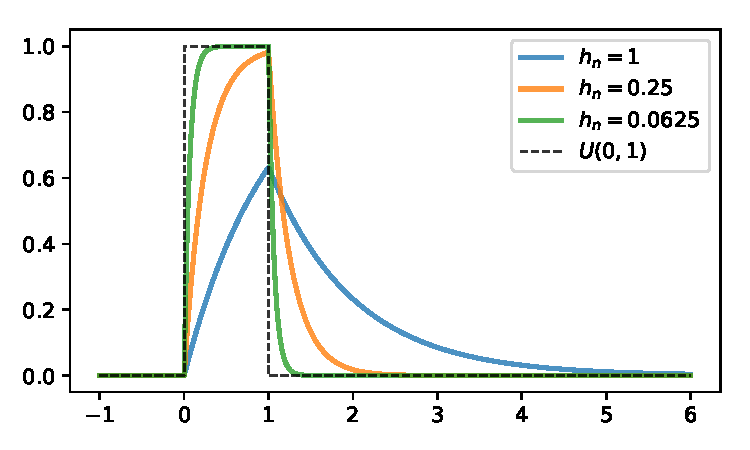
\includegraphics[width=0.5\linewidth]{figs/duda_ch4_prob3_b}
\caption{Plot of $\bar{p}(x)$ versus $x$ for $a=1$ and $h=1$, $1/4$ and $1/16$.}
\label{fig:duda_ch4_prob3_b}
\end{figure}

# The bias is $\E(p(x) - \hat{p}(x)) = p(x) - \bar{p}(x)$, and we obtain the relative bias (in percentage) by diving with $p(x)$ so that
\begin{equation*}
	\operatorname{bias}(x) = \frac{\abs{p(x) - \bar{p}(x)}}{p(x)}
	= \frac{\frac{1}{a} - \bar{p}(x)}{\frac{1}{a}} = 1 - ap(x) = e^{-x / h_n}.
\end{equation*}
The bias is decreasing on $0 < x < a$, so if we want the bias to be less than 0.01 on $99\%$ of the interval, it amounts to requiring that
\begin{equation*}
	\operatorname{bias} \left( \frac{a}{100} \right) = 0.01 
	\quad \Leftrightarrow \quad \exp \left( - \frac{a}{100 h_n} \right) = 0.01.
\end{equation*}
Solving this for $h_n$ yields $h_n = a / (100 \ln 100)$.


# When $a=0$, $h_n$ becomes $h_n = 1 / (100 \ln 100) \approx 0.0022$.
See figure \ref{fig:duda_ch4_prob3_d} for a plot.
Although it is hard to tell exactly from the plot, observe that when $x = 0.01$, the relative bias is indeed close to $0.01$ so that $\bar{p}(0.01) = 0.99$.


\begin{figure}[ht!]
\centering
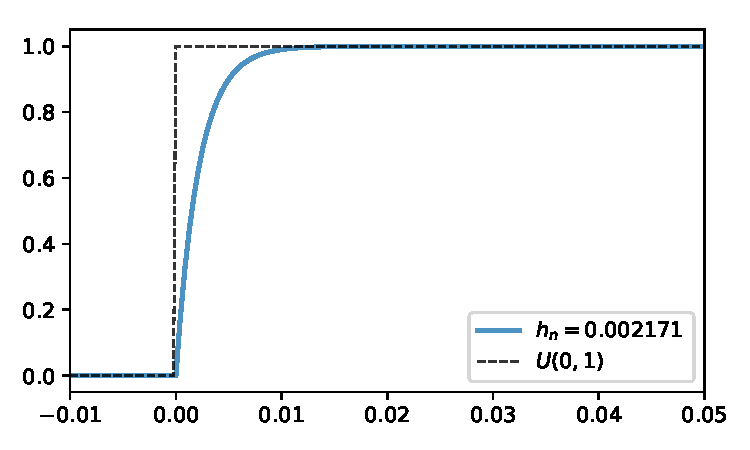
\includegraphics[width=0.5\linewidth]{figs/duda_ch4_prob3_d}
\caption{Plot accompanying problem 4.3d).}
\label{fig:duda_ch4_prob3_d}
\end{figure}

\end{easylist}


\subsubsection*{Problem 4.17}
We assume that $p(\omega_i) = 1/ c$ and $p(\vect{x} \mid \omega_i) = p(\vect{x})$.
In this case, for any point $\vect{x}$, any guess is as good as any other, and the Bayes error rate is clearly
\begin{equation*}
	P^* = \frac{c-1}{c}.
\end{equation*}
To prove that the bound
\begin{equation}
\label{eqn:ch4_problem17}
	P \leq P^* \left( 2 - \frac{c}{c - 1}P^* \right)
\end{equation}
is achieved, we calculate the error rate $P$.
In the following calculation, we use the fact that $p(\vect{x} \mid \omega_i) = p(\vect{x})$ and $\int p( \vect{x}) \, d\vect{x} = 1$.
We observe that
\begin{align*}
	P &= \int \left[ 1 - \sum_{i=1}^{c} P^2 \left( \omega_i \mid \vect{x} \right) \right] p( \vect{x}) \, d\vect{x} \\
	&= \int \left[ 1 - \sum_{i=1}^{c}  \left( \frac{p(\vect{x} \mid \omega_i) P( \omega_i) }{p(\vect{x})} \right)^2 \right] p( \vect{x}) \, d\vect{x} \\
	&= \int \left[ 1 - \sum_{i=1}^{c} P^2( \omega_i) \right] p( \vect{x}) \, d\vect{x} \\
	&= \left[ 1 - \sum_{i=1}^{c} \frac{1}{c^2} \right]  \int  p( \vect{x}) \, d\vect{x} \\
	&= 1 - c \frac{1}{c^2} = \frac{c-1}{c}.
\end{align*}

In other words, $P^*$ and $P$ are equal. 
When we substitute $P^*$ and $P$ into equation \eqref{eqn:ch4_problem17}, we see that the bound is achieved since 
\begin{equation*}
	P \leq P^* \left( 2 - \frac{c}{c - 1}P^* \right) 
	\quad  \Rightarrow \quad
	\frac{c-1}{c} \leq \frac{c-1}{c} \left( 2 - \frac{c}{c-1} \frac{c-1}{c}  \right) = \frac{c-1}{c},
\end{equation*}
which completes the proof.



\subsubsection*{Problem 4.27}
\begin{easylist}[enumerate]
\ListProperties(Space=\listSpace, Space*=\listSpace, Numbers1=l, FinalMark1={)})
# TODO

\begin{table}[ht!]
	\centering
	\caption{Ranked order of combinations of words for problem 4.27.}
	\begin{tabular}{@{}lll@{}} \toprule
	Word 1	& Word 2 & $D_\text{Tantimoto}$ \\ \midrule
	\texttt{pots} & \texttt{stop} &  0.0 \\ 
	\texttt{pattern} & \texttt{elementary} &  0.444 \\ 
	\texttt{pattern} & \texttt{pat} &  0.5 \\ 
	\texttt{taxonomy} & \texttt{elementary} &  0.5 \\ 
	\texttt{pat} & \texttt{pots} &  0.6 \\ 
	\texttt{pat} & \texttt{stop} &  0.6 \\ 
	\texttt{pattern} & \texttt{taxonomy} &  0.7 \\ 
	\texttt{pattern} & \texttt{pots} &  0.75 \\ 
	\texttt{pattern} & \texttt{stop} &  0.75 \\ 
	\texttt{pat} & \texttt{taxonomy} &  0.75 \\ 
	\texttt{pat} & \texttt{elementary} &  0.778 \\ 
	\texttt{pots} & \texttt{taxonomy} &  0.778 \\ 
	\texttt{stop} & \texttt{taxonomy} &  0.778 \\ 
	\texttt{pots} & \texttt{elementary} &  0.909 \\ 
	\texttt{stop} & \texttt{elementary} &  0.909 \\  \bottomrule
	\end{tabular}
	\label{table:problem_4_17}
\end{table}


# TODO
\end{easylist}


\subsubsection*{Problem 4.13}
\begin{easylist}[enumerate]
	\ListProperties(Space=\listSpace, Space*=\listSpace, Numbers1=l, FinalMark1={)})
	# $D(x, x_1) = \frac{4}{3} \left( x^3 - 3x + 2	 \right)$
\end{easylist}




\clearpage
\subsection{Linear discriminant functions}

\subsubsection*{Problem 5.4}
\begin{easylist}[enumerate]
	\ListProperties(Space=\listSpace, Space*=\listSpace, Numbers1=l, FinalMark1={)})
	# We wish to solve the problem
	\begin{align*}
	\underset{\vect{x}}{\operatorname{minimize}} \, & \norm{\vect{x} - \vect{x}_a}^2 =
		\vect{x}_a^T \vect{x}_a - 2\vect{x}^T \vect{x}_a + \vect{x}^T \vect{x} \\
		\text{subject to } \, & g(\vect{x}) = \vect{\omega}^T \vect{x} + \omega_0 = 0.
	\end{align*}
	To accomplish this, we start by constructing the Lagrange function
	\begin{equation*}
		L(\vect{x}, \lambda) = \vect{x}_a^T \vect{x}_a - 2\vect{x}^T \vect{x}_a + \vect{x}^T \vect{x} - \lambda( \vect{\omega}^T \vect{x} + \omega_0 - 0 ),
	\end{equation*}
	which we differentiate with respect to $\vect{x}$ and $\lambda$ to obtain:
	\begin{align*}
		L_{\vect{x}} &= -2 \vect{x}_a + 2 \vect{x} - \lambda \vect{\omega} = 0 \\
		L_\lambda &= \vect{\omega}^T \vect{x} + \omega_0 = 0
	\end{align*}
	We wish to solve these equations for $\vect{x}$.
	
	Solving the first equation for $\vect{x}$ yields $\vect{x} = \lambda \vect{\omega} / 2 + \vect{x}_a$.
	This is all well and good, but we need $\lambda$ too.
	If we left-multiply by $\vect{\omega}^T$ and compare with the second equation, we observe that
	\begin{equation*}
		\vect{\omega}^T \vect{x} 
		= -\omega_0 \quad \text{and} 
		\quad 
		\vect{\omega}^T \vect{x} 
		= 
		\frac{\norm{\vect{\omega}}^2 \lambda}{2} + \vect{\omega}^T \vect{x}_a.
	\end{equation*}
	This implies that
	\begin{equation*}
		-\omega_0 =  \frac{\norm{\vect{\omega}}^2 \lambda}{2} + \vect{\omega}^T \vect{x}_a \quad \Leftrightarrow \quad \lambda = - \frac{2}{\norm{\vect{\omega}}^2}\left( \omega_0 + \vect{\omega}^T \vect{x}_a \right),
	\end{equation*}
	and substituting this into $\vect{x} = \lambda \vect{\omega} / 2 + \vect{x}_a$ yields the optimal answer
	\begin{equation}
	\label{eqn:ch5_prob4}
		\vect{x}^* = -\frac{\vect{\omega}}{\norm{\vect{\omega}}^2} \left( \vect{\omega}^T \vect{x}_a + \omega_0 \right) + \vect{x}_a = - \frac{\vect{\omega}}{\norm{\vect{\omega}}^2} g(\vect{x}_a) + \vect{x}_a.
	\end{equation}
	Inserting this into $\norm{\vect{x}^* - \vect{x}_a}$ yields 
	\begin{equation*}
		\norm{\vect{x}^* - \vect{x}_a}=
		\norm{\frac{\vect{\omega}}{\norm{\vect{\omega}}^2} g(\vect{x}_a)}
		= \frac{\abs{g(\vect{x}_a)}}{\norm{\vect{\omega}}}.
	\end{equation*}
	
	# The projection onto the plane is the minimizer $\vect{x}^*$ from equation \eqref{eqn:ch5_prob4} in the previous problem, so we immediately see that 
	\begin{equation*}
	\vect{x}^* = -\frac{\vect{\omega}}{\norm{\vect{\omega}}^2} \left( \vect{\omega}^T \vect{x}_a + \omega_0 \right) + \vect{x}_a = - \frac{\vect{\omega}}{\norm{\vect{\omega}}^2} g(\vect{x}_a) + \vect{x}_a
	=  
	\vect{x}_a - \frac{g(\vect{x}_a)}{\norm{\vect{\omega}}^2}  \vect{\omega},
	\end{equation*}
	which is what we were required to show.
\end{easylist}

\subsubsection*{Problem 5.13}
We wish to choose $\eta(k)$ to minimize the quadratic function
\begin{equation*}
	J \left( \vect{a}(k+1)  \right)
	\simeq
	J \left( \vect{a}(k)  \right)
	-
	\eta(k) \norm{\nabla \vect{J}}^2
	+
	\frac{1}{2} \eta^2(k) \nabla \vect{J}^T \vect{H} \nabla \vect{J}.
\end{equation*}
Differentiating and setting equal to zero yields
\begin{equation*}
	\frac{\partial J \left( \vect{a}(k+1)  \right)}{\partial \eta(k)}
	=
	-
	\norm{\nabla \vect{J}}^2
	+
	\eta(k) \nabla \vect{J}^T \vect{H} \nabla \vect{J} = 0,
\end{equation*}
and solving this for $\eta(k)$ yields the desired answer
\begin{equation*}
	\eta(k) = \frac{\norm{\nabla \vect{J}}^2}{\nabla \vect{J}^T \vect{H} \nabla \vect{J}}.
\end{equation*}

\subsubsection*{Problem 5.15}
If $\alpha > \beta^2 / 2 \gamma$, then $-2 \alpha \gamma +\beta^2 < 0$ and 
\begin{equation*}
	\norm{\vect{a}(k+1) - \alpha \hat{\vect{a}}}^2 
	\leq
	\norm{\vect{a}(k) - \alpha \hat{\vect{a}}}^2 - 2 \alpha \gamma +\beta^2
\end{equation*}
represents error which decreases at each step.
After $k$ corrections we obtain
\begin{equation*}
\norm{\vect{a}(k+1) - \alpha \hat{\vect{a}}}^2 
\leq
\norm{\vect{a}(1) - \alpha \hat{\vect{a}}}^2 + k(-2 \alpha \gamma +\beta^2),
\end{equation*}
and the error is zero when $\norm{\vect{a}(1) - \alpha \hat{\vect{a}}}^2 + k_0(-2 \alpha \gamma +\beta^2) = 0$, which implies that
\begin{equation*}
	k_0 = \frac{\norm{\vect{a}(1) - \alpha \hat{\vect{a}}}^2}{2 \alpha \gamma - \beta^2}.
\end{equation*}
This is what we were asked to show.

\subsubsection*{Problem 5.21}
To ease the notation, let us write $\vect{m} := \vect{m}_1 - \vect{m}_2$\footnote{This definition of $\vect{m}$ is not the same as the one used in the book, where $\vect{m}$ is the grand mean.}.
Staring with equation (53) from the book, we left-multiply by the bracketed term to isolate $\vect{w}$ as 
\begin{equation}
\label{eqn:ch5_prob21}
	\vect{w} = \left[ \frac{1}{n} \vect{S}_W + \frac{n_1 n_2}{n^2} \vect{m} \vect{m}^T \right]^{-1} \vect{m}.
\end{equation}
Recall from problem 3.36 that the Sherman-Morrison-Woodbury matrix identity is 
\begin{equation*}
	\left(\vect{A} + \vect{x}\vect{y}^T\right)^{-1} =
	\vect{A}^{-1} - \frac{\vect{A}^{-1} \vect{x} \vect{y}^t \vect{A}^{-1}}{1 + \vect{y}^T \vect{A}^{-1} \vect{x}}.
\end{equation*}
We now apply the identity to the bracketed term in equation \eqref{eqn:ch5_prob21}.
In doing so, we identify 
\begin{equation*}
	\vect{A} \cong \frac{1}{n} \vect{S}_W 
	\quad \quad \text{and} \quad \quad
	\vect{x}\vect{y}^T \cong \frac{n_1 n_2}{n^2} \vect{m} \vect{m}^T.
\end{equation*}
Applying the matrix identity, we obtain
\begin{align*}
	\vect{w} &= \left[ n \vect{S}_W^{-1} - \frac{
		n^2 \left( \frac{n_1 n_2}{n^2} \right)
		\vect{S}_W^{-1} \vect{m} \vect{m}^T \vect{S}_W^{-1}
		}{
		1 + n \left( \frac{n_1 n_2}{n^2} \right) \vect{m}^T \vect{S}_W^{-1} \vect{m} 
		}  \right] \vect{m} \\
		&=
		n \vect{S}_W^{-1}\vect{m} - \frac{
			n \left( \frac{n_1 n_2}{n} \right)
			\vect{S}_W^{-1} \vect{m} \vect{m}^T \vect{S}_W^{-1}\vect{m}
		}{
		1 +  \left( \frac{n_1 n_2}{n} \right) \vect{m}^T \vect{S}_W^{-1} \vect{m} 
	}.
\end{align*}
To simplify the notation and remind ourselves that some of these quantities are mere scalars, let us denote $a:= n_1 n_2 / n$ and $b := \vect{m}^T \vect{S}_W^{-1} \vect{m} $.
We simplify and factor our $n \vect{S}_W^{-1} \vect{m}$ to obtain
\begin{equation*}
	\vect{w} = n \vect{S}_W^{-1}\vect{m} - \frac{
		n a
		\vect{S}_W^{-1} \vect{m} b
	}{
	1 +  a b }
	=
	n \vect{S}_W^{-1} \vect{m} \left[ 1  - \frac{ab}{1 + ab} \right]
	=
	n \vect{S}_W^{-1} \vect{m} \left[ 1  + ab \right]^{-1}.
\end{equation*}
Recalling now that $a:= n_1 n_2 / n$ and $b := \vect{m}^T \vect{S}_W^{-1} \vect{m} $, we have accomplished the goal.
The result is that
\begin{equation*}
	\vect{w} = n \vect{S}_W^{-1} \vect{m} \alpha = n \vect{S}_W^{-1} \vect{m} \big[ 1 + \underbrace{\left( \frac{n_1 n_2}{n} \right)}_a \underbrace{\vect{m}^T \vect{S}_W^{-1} \vect{m}}_b \big]^{-1},
\end{equation*}
which shows that $\alpha$ is indeed given by the quantity in the problem statement.

\subsubsection*{Problem 5.25}
\begin{easylist}[enumerate]
\ListProperties(Space=\listSpace, Space*=\listSpace, Numbers1=l, FinalMark1={)})

# We supply a proof by induction: we first show the base case, and then the inductive step.

\textbf{The base case} is verified by checking that the relation holds for $\eta^{-1}(2) = \eta^{-1}(1) + y_1^2$.
This is true, since it implies
\begin{equation*}
	\eta(2) = \frac{1}{\eta^{-1}(1) + y_1^2}
	= \frac{\eta(1)}{1 + \eta(1) y_1^2}
	= \frac{\eta(1)}{1 + \eta(1) \sum_{i=1}^{1}y_i^2},
\end{equation*}
which is clearly the given formula for $k = 2$.

In \textbf{the inductive step} we assume that the relation holds for $\eta(k)$, and show that this implies that it holds for $\eta(k+1)$ too.
The required algebra is
\begin{align*}
	\eta^{-1}(k+1) &= \eta^{-1}(k) + y_k^2 \\
&= \left( \frac{\eta(1)}{1 + \eta(1) \sum_{i=1}^{k-1}y_i^2 }  \right)^{-1} + y_k^2 \\
&= \frac{1 + \eta(1) \sum_{i=1}^{k-1}y_i^2}{\eta(1) } + \frac{\eta(1)}{\eta(1)}y_k^2 \\
&= \frac{1 + \eta(1) \sum_{i=1}^{k}y_i^2}{\eta(1)}.
\end{align*}
Inverting this shows that $\eta(k+1) = \eta(1) / \left( 1 + \eta(1) \sum_{i=1}^{k}y_i^2 \right)$, as required.



# To show why the sequence of coefficients will satisfy the sums, we will first bound the terms, and the convert the problems to integrals.

If $0 < a \leq y_i^2 \leq b < \infty$ for every $i$, then the sum is bounded by
\begin{equation*}
	a(k-1) \leq \sum_{i=1}^{k-1} y_i^2 \leq b(k-1),
\end{equation*}
and this in turn implies the expression $\eta(k)$ that may be bounded by
\begin{equation*}
	\frac{\eta(1)}{1 + \eta(1) b(k-1)} \leq \eta(k) \leq\frac{\eta(1)}{1 + \eta(1) a(k-1)}.
\end{equation*}

To show that $\sum \eta(k) \to \infty$, we note that $\sum \eta(k) \simeq \lim_{\alpha \to \infty} \int_{x=1}^{x=\alpha} \eta(x) \, dx $.
We observe that the integral
\begin{equation*}
	\lim_{\alpha \to \infty} \int_{x=1}^{x=\alpha} \frac{\eta(1)}{1 + \eta(1)(x-1)b} \, dx 
	= 
	\lim_{\alpha \to \infty} \left. \frac{1}{b} \ln \abs{u} \right|_{u=1}^{u=1 + \eta(1) (\alpha - 1)b}
\end{equation*}
diverges for any value of $b$, where we used the substitution $u = 1 + \eta(1)(x-1)b$.
Since $b$ represents the maximal value of the terms $\eta(k)$, any other value of $y_i^2$ will diverge too, and the sum $\sum \eta(k)$ diverges to infinity.

To show that $\sum \eta^2(k) \to L < \infty$, we again use $\sum \eta^2(k) \simeq \lim_{\alpha \to \infty} \int_{x=1}^{x=\alpha} \eta^2(x) \, dx $.
Now the integral converges, since for any value of $a$ the integral
\begin{equation*}
\lim_{\alpha \to \infty} \int_{x=1}^{x=\alpha} \frac{\eta^2(1)}{(1 + \eta(1)(x-1)b)^2} \, dx 
= 
\lim_{\alpha \to \infty} \left. \frac{\eta(1)}{bu} \right|_{u=1 + \eta(1) (\alpha - 1)a}^{u=1} \leq \frac{\eta(1)}{b}
\end{equation*}
diverges, and $a$ represents the maximal bound on $\eta(k)$. 
The sum $\sum \eta(k)$ diverges to infinity, for any $0 < a \leq y_i^2 \leq b < \infty$.
\end{easylist}




\subsubsection*{Problem 5.27}
\begin{easylist}[enumerate]
\ListProperties(Space=\listSpace, Space*=\listSpace, Numbers1=l, FinalMark1={)})
# The data points are plotted in figure \ref{fig:duda_ch5_prob27} on page \pageref{fig:duda_ch5_prob27}, and as seen they are not linearly separable.


\begin{figure}[ht!]
	\centering
	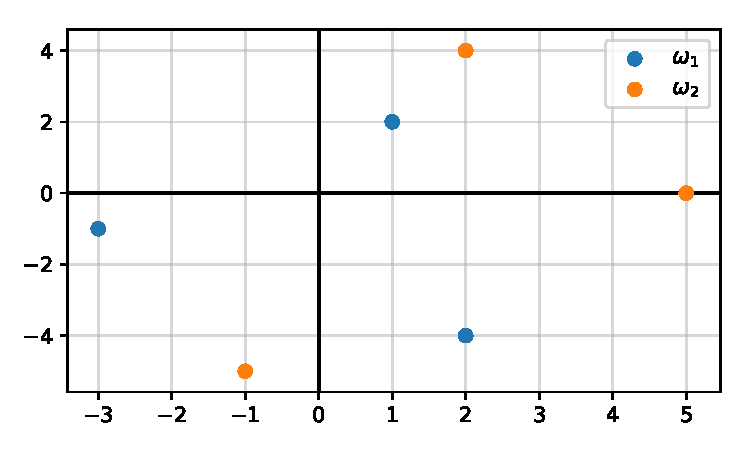
\includegraphics[width=0.5\linewidth]{figs/duda_ch5_prob27}
	\caption{Graf accompanying problem 5.27.}
	\label{fig:duda_ch5_prob27}
\end{figure}


# From equation (95) we observe that the optimal choice of $\eta$ is given by

\begin{equation*}
	\eta(k) = \frac{\norm{\vect{Y}^T \abs{\vect{e}(k)}}^2}
	{\norm{\vect{Y}\vect{Y}^T \abs{\vect{e}(k)}}^2}
	= \frac{\vect{e}^T \vect{Y} \vect{Y}^T \vect{e}}
	{\vect{e}^T \vect{Y} \vect{Y}^T \vect{Y} \vect{Y}^T \vect{e}}.
\end{equation*}
This value varies from loop to loop, depending on $\vect{e}$.
For this specific data set, the value of $\vect{Y}$ and $\vect{Y} \vect{Y}^T$ are given in equation \eqref{eqn:chapter5_prob27}.

\begin{gather*}
\label{eqn:chapter5_prob27}
	\vect{Y} = \left(\begin{matrix}
	1.0 & 1.0 & 2.0\\1.0 & 2.0 & -4.0\\1.0 & -3.0 & -1.0\\-1.0 & -2.0 & -4.0\\-1.0 & 1.0 & 5.0\\-1.0 & -5.0 & 0.0
	\end{matrix}\right)
	\\
	\vect{Y} \vect{Y}^T = 
	\left(\begin{matrix}
	6.0 & -5.0 & -4.0 & -11.0 & 10.0 & -6.0\\-5.0 & 21.0 & -1.0 & 11.0 & -19.0 & -11.0\\-4.0 & -1.0 & 11.0 & 9.0 & -9.0 & 14.0\\-11.0 & 11.0 & 9.0 & 21.0 & -21.0 & 11.0\\10.0 & -19.0 & -9.0 & -21.0 & 27.0 & -4.0\\-6.0 & -11.0 & 14.0 & 11.0 & -4.0 & 26.0
	\end{matrix}\right)
\end{gather*}

\begin{figure}[ht!]
	\centering
	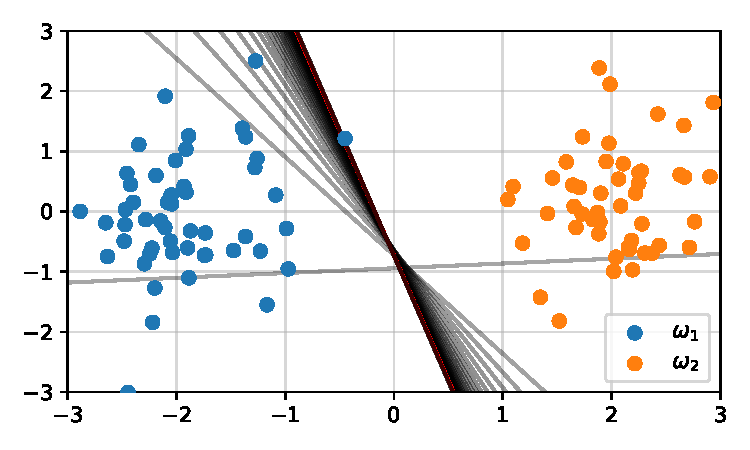
\includegraphics[width=0.5\linewidth]{figs/duda_ch5_prob27_b}
	\caption{Convergence of the Ho Kashyap algorithm.}
	\label{fig:duda_ch5_prob27_b}
\end{figure}

\end{easylist}


\subsubsection*{Problem 5.29}
To show that there always exists a mapping to a higher dimensional space which leaves points from two classes linearly separable, we will explicitly provide such a mapping.
The mapping would be very inefficient in practice, but provides a constructive proof.

Observe first that to apply a linear classifier to points where data from one class is close to the origin, a function such as $y = \phi (\vect{x}) = \exp(- \vect{x}^T \vect{x})$ may be used.
This leave the data linearly separable in the new space, as illustrated in figure \ref{fig:1024px_Kernel_trick_idea_svg_wikipedia}.
Below we will extend this idea by introducing many distinct mappings $\phi (\vect{x})$.
\begin{figure}
	\centering
	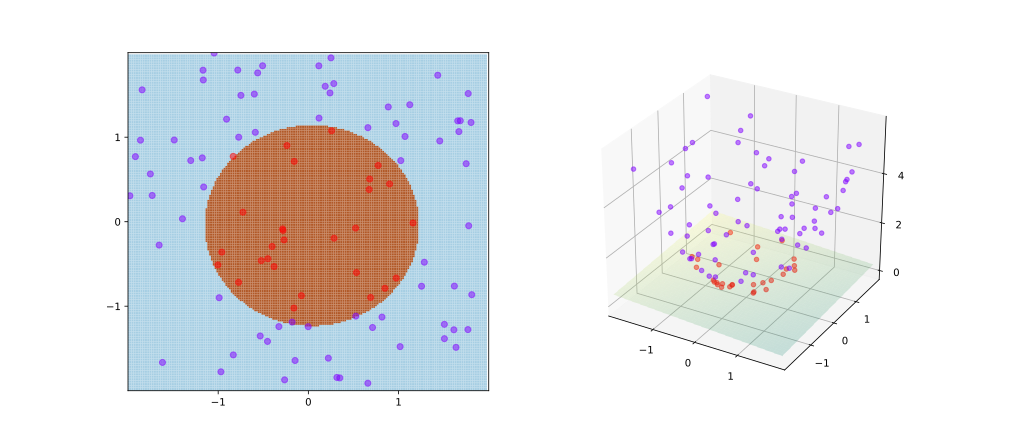
\includegraphics[width=0.85\linewidth]{figs/1024px_Kernel_trick_idea_svg_wikipedia}
	\caption{Using a kernel to raise points in a new dimension. Source: \url{https://commons.wikimedia.org/wiki/File:Kernel_trick_idea.svg}}
	\label{fig:1024px_Kernel_trick_idea_svg_wikipedia}
\end{figure}

Consider now points $\D = \left\{ \vect{x}_1, \vect{x}_2, \dots, \vect{x}_N \right\}$ in $\R^d$.
Assume that some points $S \subseteq \D$ belong to $\omega_1$, and that we know exactly which points. 
If we know which points belong to  $\omega_1$, then a kernel density estimate  (Parzen window) such as
\begin{equation*}
	y  = \operatorname{Parzen}(S) = \frac{1}{\abs{S}}\sum_{\vect{x}_i \in S} \frac{1}{h} \phi \left( \frac{\vect{x} - \vect{x}_i}{h} \right)
\end{equation*}
with a sufficiently small value of the bandwidth $h$ will raise these points in the new $y$ feature space.
When $h \ll 1$, neighboring points not belonging to $\omega_1$ will be unaffected.
A plane such as $y = 0.1$ will then perfectly separate the points.

Since we do not know the true subset $S \subseteq \D$, we can apply this transformation on \emph{every} subset of $\D$ (the \emph{power set} of $\D$).
There are $2^{\abs{S}}$ such subsets.
We use
\begin{equation*}
	\vect{y} = 
	\begin{pmatrix}
	\vect{x} & \operatorname{Parzen}(S_1) & \operatorname{Parzen}(S_1) & \dots & \operatorname{Parzen}(S_{2^{\abs{S}}})
	\end{pmatrix}
\end{equation*}
to map $\vect{x} \in \R^d$ to a $d + 2^{\abs{S}$ space.
In other words: if $\left\{ \vect{x_1} \right\}$ is ``raised'' in one new feature dimension, $\left\{ \vect{x_1}, \vect{x_2} \right\}$ in another, $\left\{ \vect{x_1}, \vect{x_3} \right\}$ in yet another, etc. for \emph{every} combination of points, then in some dimension in the feature space the points are linearly separable.






\subsubsection*{Problem 5.32}
\begin{easylist}[enumerate]
\ListProperties(Space=\listSpace, Space*=\listSpace, Numbers1=l, FinalMark1={)})
# The plot is show in figure \ref{fig:duda_ch5_prob32}.
By inspection the weight vector is 
\begin{equation*}
	\vect{a} = (a_0, a_1, a_2)= (-1.5, 1, 1).
\end{equation*}
This corresponds to the line $y = 1.5 - x$.
The optimal margin is the distance from the line $y = 1.5 - x$ to a point, say $(1,1)$, and this distance is $\sqrt{2}/4 \approx 0.3536$.

\begin{figure}[ht!]
	\centering
	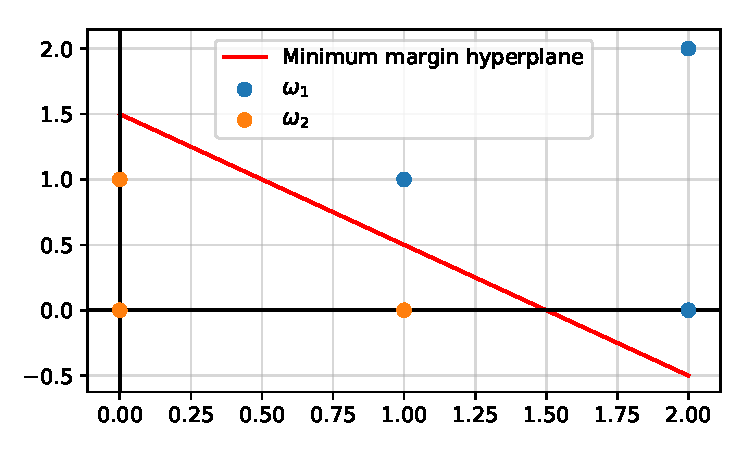
\includegraphics[width=0.5\linewidth]{figs/duda_ch5_prob32}
	\caption{Plot related to problem 5.32a).}
	\label{fig:duda_ch5_prob32}
\end{figure}

# From inspection there are four support vectors, they are
\begin{align*}
	(0, 1)^T \quad & \quad (1, 0)^T \\
	(1, 1)^T \quad & \quad (2, 0)^T.
\end{align*}

# This laborious computation is omitted.


\end{easylist}




\subsubsection*{Problem 5.33}
\begin{easylist}[enumerate]
\ListProperties(Space=\listSpace, Space*=\listSpace, Numbers1=l, FinalMark1={)})
# The optimization problem
\begin{equation}
\label{eqn:ch5_problem_33_1}
	L(\vect{a}, \vect{\alpha}) = \frac{1}{2} \norm{\vect{a}}^2 -
	\sum_{k=1}^{n} \alpha_k \left[ z_k \vect{a}^T \vect{y}_k - 1 \right]
\end{equation}
has a solution which is a saddle point since we wish to maximize with respect to $\vect{\alpha}$ and minimize with respect to $\vect{a}$.

# Here I believe there to be a slight error in the text, which might lead to confusion.
In the initial pages of the chapter, the distance from a point to a hyperplane is given by $r = (\vect{\omega}^T \vect{x} + \omega_0) / \norm{\vect{\omega}}$, and this is indeed correct.

In the context of SVMs, however, the distance is said to be 
\begin{equation*}
	\frac{g(y)}{\norm{\vect{a}}}
	=
	\frac{\vect{a} ^T \vect{y}}{\norm{\vect{a}}}
	=
	\frac{(\omega_0, \vect{a}') (1, \vect{y}')^T}{\norm{\vect{a}}}
	=
	\frac{\vect{a}'\,^T\vect{y} + \omega_0}{\norm{\vect{a}}},
\end{equation*}
which is different because $\vect{a}$ is in the denominator, not $\vect{a}'$.
Amending equation \eqref{eqn:ch5_problem_33_1} with this information, the $\frac{1}{2} \norm{\vect{a}}^2$ should be replaced by $\frac{1}{2} \norm{\vect{a}'}^2$, i.e. dropping $\vect{a}_0 = \omega_0$.
If we do this and differentiate with respect to the first component of $\vect{a}$, we obtain
\begin{equation*}
	\frac{\partial L(\vect{a}, \vect{\alpha})}{\partial \vect{a}_0}
	=
	\sum_k \alpha_k^* z_k \vect{y}_0 = 0,
\end{equation*}
which gives the desired result since $\vect{y}_0 = 1$ due to the augmentation of the vector.

# To prove this, we differentiate with respect to $\vect{a}$ and obtain
\begin{equation*}
\frac{\partial L(\vect{a}, \vect{\alpha})}{\partial \vect{a}}
=
\vect{a}^* - \sum_k \alpha_k^* z_k \vect{y}_k = 0.
\end{equation*}

# If the Lagrange multiplier (or \emph{undetermined multiplier}) $\alpha_k^*$ is zero, then it's said to be \emph{inactive}.
At the optimum, the constraint is not used.
The optimum of $L(\vect{a}, \vect{\alpha})$ is the same with or without this constraint.

If the Lagrange  multiplier $\alpha_k^*$ is non-zero, then it's said to be \emph{active}.
The constrained solution is different from the unconstrained solution, and the optimum lies on the boundary of the constraint.
Since $\alpha_k^* z_k \vect{y}_k \geq 1$ in the feasible region, the optimal solution is on the boundary if $\alpha_k^* z_k \vect{y}_k = 1$, but then  $\alpha_k^*$ is non-zero since the constraint is active.

In conclusion, either $\alpha_k^* z_k \vect{y}_k = 1$ if the constraint is active, or $\alpha_k^* = 0$ if the constraint is inactive.
This is one of the Karush–Kuhn–Tucker (KKT) conditions, and it may be expressed as
\begin{equation*}
	\alpha_k^* \left[ \alpha_k^* z_k \vect{y}_k - 1 \right] = 0 \qquad k = 1 , \dots, n.
\end{equation*}

# Simply multiply the brackets in equation \eqref{eqn:ch5_problem_33_1} from subproblem a).
\begin{equation*}
L(\vect{a}, \vect{\alpha}) = \frac{1}{2} \norm{\vect{a}}^2 -
\sum_{k=1}^{n} \alpha_k \left[ z_k \vect{a}^T \vect{y}_k - 1 \right]
=
\frac{1}{2} \norm{\vect{a}}^2 -
\sum_{k=1}^{n} \alpha_k  z_k \vect{a}^T \vect{y}_k 
+
\sum_{k=1}^{n} \alpha_k 
\end{equation*}

# Using $\vect{a}^* = \sum_j \alpha_j^* z_j \vect{y}_j$ we observe that
\begin{align*}
	L(\vect{\alpha}) &= 
	\frac{1}{2} \norm{\vect{a}^*}^2 -
	\sum_{k=1}^{n} \alpha_k  z_k \vect{a}^{*T} \vect{y}_k 
	+
	\sum_{k=1}^{n} \alpha_k \\
	&= 
	\frac{1}{2} 
	\left(\sum_j \alpha_j^* z_j \vect{y}^T_j\right)
	\left(\sum_k \alpha_k^* z_k \vect{y}_k\right)
	 -
	\sum_{k=1}^{n} \alpha_k  z_k 
	\left(\sum_j \alpha_j^* z_j \vect{y}^T _j\right)
	\vect{y}_k 
	+
	\sum_{k=1}^{n} \alpha_k 
\end{align*}
and since the first and second terms are equal, we obtain
\begin{equation*}
-
\frac{1}{2} 
\left(\sum_j \alpha_j^* z_j \vect{y}^T_j\right)
\left(\sum_k \alpha_k^* z_k \vect{y}_k\right)
+
\sum_{k=1}^{n} \alpha_k 
= 
-
\frac{1}{2} 
\sum_j \sum_k \alpha_j^* \alpha_k^* z_j z_k \vect{y}_j^T \vect{y}_k
+
\sum_{k=1}^{n} \alpha_k 
\end{equation*}
as desired.
We have formulated the problem as a maximization over $L(\vect{\alpha})$.
\end{easylist}




























\clearpage
\subsection{Multilayer Neural Networks}

\subsubsection*{Problem 6.5}
\begin{easylist}[enumerate]
\ListProperties(Space=\listSpace, Space*=\listSpace, Numbers1=l, FinalMark1={)})
# DONE
\end{easylist}

\subsubsection*{Problem 6.10}
\begin{easylist}[enumerate]
	\ListProperties(Space=\listSpace, Space*=\listSpace, Numbers1=l, FinalMark1={)})
	# Simple calculus shows that when $f(x) = 1 /(1 + e^{ax} )$, then the derivative may be expressed in terms of the function as
	\begin{equation*}
		f'(x) = -a e^{ax} f^2(x).
	\end{equation*}
	
	# We'll study $f(x) = a (1 - e^{-2bx}) / (1 + e^{-2bx})$, and here it pays off to ease notation somewhat.
	Letting $g(x) := e^{-2bx}$, we have $g'(x) = -2b g(x)$ and
	\begin{equation*}
		f(x) = a \frac{1 - e^{-2bx}}{1 + e^{-2bx}} :=
		a \frac{1 - g(x)}{1 + g(x)} =  a (1 - g(x)) (1 + g(x))^{-1}.
	\end{equation*}
	We differentiate to obtain 
	\begin{align*}
		f'(x) &=  \frac{-a g'(x) (1 + g(x)) - ag'(x) (1 - g(x))}{(1 + g(x))^2} \\
		&= \frac{4 ab g(x)}{(1 + g(x))^2} = \underbrace{a \frac{1 - g(x)}{1 + g(x)}}_{f'(x)} \frac{4bg(x)}{(1 - g(x)) (1 + g(x))}.
	\end{align*}
	Substituting back $g(x) := e^{-2bx}$, we see that  the derivative may be expressed in terms of the function as
	\begin{equation*}
		f'(x) = f(x) \frac{4 b  e^{-2bx}}{1 - e^{-4bx}}.
	\end{equation*}
\end{easylist}

\subsubsection*{Problem 6.13}
\begin{easylist}[enumerate]
	\ListProperties(Space=\listSpace, Space*=\listSpace, Numbers1=l, FinalMark1={)})
	# DONE
\end{easylist}

\subsubsection*{Problem 6.15}
\begin{easylist}[enumerate]
	\ListProperties(Space=\listSpace, Space*=\listSpace, Numbers1=l, FinalMark1={)})
	# sdf
\end{easylist}

\subsubsection*{Problem 6.21}
\begin{easylist}[enumerate]
	\ListProperties(Space=\listSpace, Space*=\listSpace, Numbers1=l, FinalMark1={)})
	# DONE
\end{easylist}

\subsubsection*{Problem 6.24}
\begin{easylist}[enumerate]
	\ListProperties(Space=\listSpace, Space*=\listSpace, Numbers1=l, FinalMark1={)})
	# DONE
\end{easylist}

\subsubsection*{Problem 6.26}
\begin{easylist}[enumerate]
	\ListProperties(Space=\listSpace, Space*=\listSpace, Numbers1=l, FinalMark1={)})
	# sdf
\end{easylist}

\subsubsection*{Problem 6.31}
\begin{easylist}[enumerate]
	\ListProperties(Space=\listSpace, Space*=\listSpace, Numbers1=l, FinalMark1={)})
	# sdf
\end{easylist}

\subsubsection*{Problem 6.37}
\begin{easylist}[enumerate]
	\ListProperties(Space=\listSpace, Space*=\listSpace, Numbers1=l, FinalMark1={)})
	# sdf
\end{easylist}

\subsubsection*{Problem 6.39}
\begin{easylist}[enumerate]
	\ListProperties(Space=\listSpace, Space*=\listSpace, Numbers1=l, FinalMark1={)})
	# If we write out the sums, we obtain
	\begin{equation*}
		f(\vect{x}) = \vect{x}^T \vect{K} \vect{x} = \sum_i \sum_j x_i K_{ij} x_j.
	\end{equation*}
	Of course, the function $f(\vect{x})$ is a mapping from a vector $\vect{x} \in \R^d$ to a real number $\R$.
	In this setting, the derivative is the gradient, i.e. $\nabla f(\vect{x}) = f'(\vect{x})$.
	To find the gradient using explicit components, we write
	\begin{gather}
		\nonumber \frac{d}{d x_k} \left( \vect{x}^T \vect{K} \vect{x} \right)  = \\ 
		\nonumber \frac{d}{d x_k} \left( \sum_i x_i \sum_j K_{ij} x_j \right)  = \\
		\label{eqn:ch6_problem39a} \frac{d}{d x_k} \left( 
		x_1 \left( \sum_j K_{1j} x_j \right) + 
		x_2 \left( \sum_j K_{2j} x_j \right) + \dots +
		x_k \left( \sum_j K_{kj} x_j \right) + \dots
		 \right).
	\end{gather}
	For every term $i \neq k$ , the derivative is $x_i K_{ik}$.
	On the $k$'th term, we apply the product rule of differentiation to obtain
	\begin{equation*}
		\frac{d}{d x_k} \left( x_k \left( \sum_j K_{kj} x_j \right) \right)=
		1 \left( \sum_j K_{kj} x_j \right) +
		x_k \left( K_{kk} \right).
	\end{equation*}
	Applying these results to the non-$k$'th terms and the $k$'th term respectively, equation \eqref{eqn:ch6_problem39a} becomes
	\begin{align*}
	\frac{d}{d x_k} \left( \vect{x}^T \vect{K} \vect{x} \right)  &=  x_1 K_{1k} + x_2 K_{2k} + x_3 K_{3k} + \dots + 
		\left(  \sum_j K_{kj} x_j  +
		x_k  K_{kk}  \right)
		+ \dots  \\
		& =  \sum_i x_i K_{ik} + \sum_j K_{kj} x_j = 
		\vect{K}^T \vect{x} + \vect{K} \vect{x} = 
		\left( \vect{K}^T + \vect{K}  \right)\vect{x},
	\end{align*}
	where the last equality follows from
	\begin{align*}
		\vect{b} = \vect{A} \vect{x} \quad &\Leftrightarrow \quad
		b_i = \sum_j A_{ij} x_j \\
		\vect{b} = \vect{A}^T \vect{x} \quad &\Leftrightarrow \quad
		b_i = \sum_j A_{ji} x_j.
	\end{align*}
	
	# Here's an approach which does not require indices, and is therefore more expedient.
	Let $f(\vect{x}) = \vect{x}^T \vect{H} \vect{x}$, where $\vect{H}$ is symmetric.
	We have
	\begin{equation*}
		f(\vect{x} + \delta \vect{x}) - f( \vect{x}) = 
		\left( \delta \vect{x} \right)^T \vect{H} \vect{x} + 
		\vect{x}^T \vect{H} \left( \delta \vect{x} \right)
		+ O \left( \norm{ \delta \vect{x} }^2 \right),
	\end{equation*}
	and when $\vect{H}$ is symmetric this becomes 
	\begin{equation*}
			f(\vect{x} + \delta \vect{x}) - f( \vect{x}) = 
			2 \vect{x}^T \vect{H} \left( \delta \vect{x} \right)
			+ O \left( \norm{ \delta \vect{x} }^2 \right).
	\end{equation*}
	So $2 \vect{x}^T \vect{H}$ is indeed the first-order approximation to  $f(\vect{x} + \delta \vect{x})$.
	The reader might react to the fact that the derivative in problem a) is a column vector, while the derivative in problem b) is a row vector.
	The gradient is really a row vector, since $\left( \nabla f(\vect{x} ) \right)^T \delta \vect{x}$ produces a real number.
	
\end{easylist}

\subsubsection*{Problem 6.42}
The weight decay rule of equation (38) in the book does not exactly lead to equation (39).
The rule multiplies the weight set by gradient descent by the factor $(1 - \epsilon)$, such that 
\begin{equation*}
	\vect{w}_{n+1} = \left( \vect{w}_{n} - \eta \nabla J(\vect{w}_n ) \right) (1 - \epsilon).
\end{equation*}
Moving the terms around a little bit, we observe that this is equivalent to
\begin{equation*}
		\vect{w}_{n+1} = \vect{w}_{n} - \eta  \underbrace{\left(
			(1 - \epsilon ) \nabla J(\vect{w}_n ) + \frac{\epsilon}{\eta} \vect{w}_n
			\right)}_{\nabla J_{ef}(\vect{w}_n)} .
\end{equation*}
Since $\nabla \vect{w}^T \vect{w} = 2 \vect{w}$, we observe that $J_{ef}(\vect{w}_n) = (1 - \epsilon ) J(\vect{w}_n ) + \epsilon \frac{1}{2 \eta} \vect{w}_n^T \vect{w}_n $.
This is a weighted average of the ordinary error function $J(\vect{w}_n )$ and the regularization term $\frac{1}{2 \eta} \vect{w}_n^T \vect{w}_n$.
We can easily verify that 
(1) when $\epsilon = 0$, everything reduces to the ordinary gradient descent with no weight decay and
(2) when $\epsilon = 1$, $\vect{w}_{n+1}$ is forever stuck at $\vect{0}$.

This also shows that equation (39) in the book is wrong with respect to equation (38), since if $\epsilon=1$ in the book, equation (38) would always set $\vect{w}_{n+1} = \vect{0}$ while optimizing equation (39) would not---it would amount to optimizing $J(\vect{w} )$ with a regularization term.





\clearpage

\subsubsection*{Problem X.YY}
\begin{easylist}[enumerate]
	\ListProperties(Space=\listSpace, Space*=\listSpace, Numbers1=l, FinalMark1={)})
	# sdf
\end{easylist}





\end{document}
